\documentclass[11pt,oneside,openany]{book}

\usepackage[T1]{fontenc}
\usepackage[utf8]{inputenc}
\usepackage{lmodern}
\usepackage{microtype}
\usepackage[a4paper,top=25mm,bottom=25mm,left=28mm,right=25mm,headheight=23pt]{geometry}
\usepackage{amsmath,amssymb,mathtools}
\usepackage{booktabs,longtable,array,tabularx,multirow}
\usepackage{graphicx}
\graphicspath{{figures/}}
\usepackage{xcolor}
\definecolor{navy}{HTML}{0B1F33}
\definecolor{slate}{HTML}{334155}
\definecolor{muted}{HTML}{64748B}
\definecolor{rulegray}{HTML}{CBD5E1}
\definecolor{lightblue}{HTML}{EFF6FF}
\definecolor{lightgray}{HTML}{F8FAFC}
\usepackage{fancyhdr}
\usepackage{titlesec}
\usepackage{enumitem}
\usepackage{setspace}
\usepackage{listings}
\usepackage{hyperref}
\usepackage{bookmark}
\usepackage[noautomatic]{imakeidx}
\usepackage{etoolbox}

\hypersetup{
  colorlinks=true,
  linkcolor=navy,
  citecolor=slate,
  urlcolor=slate,
  pdftitle={Finance and Quantitative Markets},
  pdfauthor={Scott Brodie Forsyth}
}

\makeindex
\setstretch{1.08}
\emergencystretch=2em
\setlength{\parindent}{0pt}
\setlength{\parskip}{5pt}
\setlist[itemize]{leftmargin=*,itemsep=2pt,topsep=3pt}
\setlist[enumerate]{leftmargin=*,itemsep=3pt,topsep=3pt}

\titleformat{\chapter}[display]
  {\normalfont\bfseries\color{navy}}
  {\filleft\Large\chaptertitlename\ \thechapter}
  {8pt}
  {\Huge\filright}
  [\vspace{5pt}\color{rulegray}\titlerule]
\titleformat{\section}{\Large\bfseries\color{navy}}{\thesection}{0.7em}{}
\titleformat{\subsection}{\large\bfseries\color{slate}}{\thesubsection}{0.7em}{}
\titlespacing*{\chapter}{0pt}{0pt}{20pt}
\titlespacing*{\section}{0pt}{16pt}{5pt}
\titlespacing*{\subsection}{0pt}{12pt}{3pt}

\pagestyle{fancy}
\setlength{\headheight}{23pt}
\fancyhf{}
\fancyhead[L]{\small\color{muted}Finance and Quantitative Markets}
\fancyhead[R]{\small\color{muted}Chapter \thechapter}
\fancyfoot[C]{\small\thepage}
\renewcommand{\headrulewidth}{0.3pt}
\renewcommand{\footrulewidth}{0pt}

\lstset{
  basicstyle=\small\ttfamily,
  keywordstyle=\color{navy}\bfseries,
  commentstyle=\color{muted}\itshape,
  stringstyle=\color{slate},
  showstringspaces=false,
  frame=single,
  rulecolor=\color{rulegray},
  backgroundcolor=\color{lightgray},
  breaklines=true,
  columns=fullflexible,
  keepspaces=true,
  numbers=left,
  numberstyle=\tiny\color{muted},
  numbersep=7pt
}

\newcommand{\R}{\mathbb{R}}
\newcommand{\E}{\mathbb{E}}
\newcommand{\Var}{\operatorname{Var}}
\newcommand{\Cov}{\operatorname{Cov}}
\newcommand{\Prob}{\mathbb{P}}
\newcommand{\dd}{\,\mathrm{d}}
\newcommand{\given}{\,|\,}
\newcommand{\floor}[1]{\left\lfloor #1 \right\rfloor}
\newcommand{\ceil}[1]{\left\lceil #1 \right\rceil}
\newcommand{\source}[1]{\par\smallskip{\footnotesize\color{muted}Source note: #1}\par}
\newcommand{\keyterm}[1]{\textbf{#1}\index{#1}}
\newcommand{\formula}[1]{\begin{equation}\label{#1}}
\newcommand{\closeformula}{\end{equation}}
\newenvironment{important}{\begin{quote}\itshape\color{slate}}{\end{quote}}
\newenvironment{worked}{\begin{quote}\small\textbf{Worked example.}\ }{\end{quote}}
\newenvironment{exerciseblock}{\begin{quote}\small\textbf{Exercises.}\ }{\end{quote}}
\newenvironment{solutionblock}{\begin{quote}\small\textbf{Solution.}\ }{\end{quote}}

\begin{document}

\hypersetup{pageanchor=false}
\begin{titlepage}
  \pagecolor{navy}
  \color{white}
  \vspace*{0.20\textheight}
  {\Huge\bfseries FINANCE\\[7pt]AND QUANTITATIVE MARKETS\par}
  \vspace{18pt}
  {\Large Value, Risk, Decisions, and Financial Systems\par}
  \vfill
  {\large Scott Brodie Forsyth\par}
  \vspace{10pt}
  {\small First edition | 17 July 2026\par}
\end{titlepage}
\nopagecolor
\color{black}
\hypersetup{pageanchor=true}

\frontmatter

\chapter*{Copyright and use}
This educational manuscript is an independent textbook. It is not investment, tax, accounting, legal, or regulatory advice. Examples are for learning and may omit facts that matter in a real transaction. A security that appears in an example is not a recommendation. Prices, returns, and simulated paths do not predict future outcomes.

The book is designed to be reproducible. Calculations in the text use either exact symbolic inputs, transparently rounded classroom inputs, or the simulated data supplied with the source package. Regulatory statements are scoped to the jurisdictions and date stated in the text. Laws, rules, products, and market conventions change; readers making real decisions should consult the relevant current authority and professional advisers.

\chapter*{How to use this book}
The first half develops the language of finance: claims, cash flows, discounting, accounting, assets, and corporate decisions. The second half adds probability, statistics, portfolio theory, derivatives, stochastic models, numerical methods, and risk. Each chapter moves through intuition, formal definitions, assumptions, worked calculations, limitations, and exercises. The Python and spreadsheet files are companion laboratories, not black boxes: every major function is short enough to inspect and test.

The symbol $t$ denotes time, $0$ is the valuation date, and $T$ is a future date unless a chapter says otherwise. Rates are annual effective rates unless a compounding frequency is written explicitly. Dollar signs in examples mean generic currency units; the methods are not tied to the United States.

\chapter*{Data, evidence, and scope}
This edition was checked on 17 July 2026. The book distinguishes three kinds of statements:

\begin{itemize}
  \item \textit{identities and derivations}, which follow from definitions and stated assumptions;
  \item \textit{empirical claims}, which are linked to published research or official data documentation; and
  \item \textit{current institutional claims}, which carry a date and a source because they can change.
\end{itemize}

The executable dataset is simulated with a fixed random seed. It is intentionally not presented as historical market performance. The source package also documents legal routes for replacing it with official observations, such as SEC XBRL financial-statement data, Treasury security documentation, or a central-bank data API, subject to the terms of each provider.

\tableofcontents
\listoffigures

\mainmatter

\chapter{Finance as Decisions Under Time and Risk}

\section{The central problem}
Finance studies how people and organisations move resources across time and uncertainty. A household saves part of current income to pay for a future education. A firm raises capital to build capacity whose cash flows arrive later. A pension fund exchanges current contributions for uncertain future benefits. A bank transforms short-term deposits into longer-term loans. These are different transactions, but each asks the same question: what is a future, risky claim worth today?

The answer cannot be a number without a context. Value depends on the timing of cash flows, their uncertainty, the alternatives available to the decision-maker, taxes and transaction costs, and the legal rights attached to the claim. A useful discipline is therefore to write down the cash-flow distribution before choosing a valuation model.

\begin{important}
Finance is not primarily the art of forecasting a single price. It is the disciplined comparison of uncertain cash flows under explicit assumptions.
\end{important}

\section{Claims, cash flows, and balance sheets}
A \keyterm{financial claim} is a contract or ownership right that entitles its holder to future cash flows or control rights. Debt normally promises specified payments and gives creditors priority in insolvency. Equity is a residual claim: shareholders receive what remains after contractual obligations, and often receive voting rights. An option gives a right, not an obligation, to transact under specified conditions.

For a claim $i$, let $C_{i,t}$ be the cash flow received by its owner at time $t$. A cash-flow vector is
\formula{cashvector}
  \mathbf{C}_i=(C_{i,0},C_{i,1},\ldots,C_{i,T}).
\closeformula
Negative values represent payments by the holder. The same transaction looks different from the issuer's perspective because the sign is reversed. A financial statement is an organised description of a firm's resources, obligations, performance, and cash movements; it is not itself a valuation.

The basic accounting identity is
\formula{balanceidentity}
  \text{Assets}=\text{Liabilities}+\text{Equity}.
\closeformula
Assets are controlled resources expected to produce benefits. Liabilities are present obligations. Equity is the residual interest. This identity is an accounting representation of claims on resources, not a guarantee that book values equal market values.

\section{Return and wealth}
Suppose an asset costs $P_0$ at the beginning of a period, pays a cash distribution $D_1$, and is worth $P_1$ at the end. The simple holding-period return is
\formula{return}
  R_1=\frac{P_1-P_0+D_1}{P_0}.
\closeformula
Here $P_0>0$ is the initial price, $P_1$ is the ending price, and $D_1$ is the cash distribution received during the period. The numerator is the investor's gain: price change plus distribution.

If wealth is compounded through periods, the terminal wealth from initial wealth $W_0$ is
\formula{wealthcompounding}
  W_T=W_0\prod_{t=1}^{T}(1+R_t).
\closeformula
The geometric average return over $T$ periods is $\left(W_T/W_0\right)^{1/T}-1$. The arithmetic average is $T^{-1}\sum_tR_t$. They answer different questions: the arithmetic mean is useful for some expected-return calculations, while the geometric mean describes the realised compound growth rate.

\begin{worked}
An asset rises from 100 to 108 and pays a distribution of 2. The holding-period return is $(108-100+2)/100=0.10$, or 10 percent. If the next period return is -10 percent, two-period wealth is $100(1.10)(0.90)=99$. The arithmetic average is 0 percent, but the compounded result is a 1 percent loss. Volatility interacts with compounding.
\end{worked}

\section{Risk is multidimensional}
Risk is not synonymous with volatility. Volatility measures dispersion of returns around a mean, but an investor may care about permanent loss, shortfall relative to liabilities, liquidity, inflation, counterparty default, model error, or the possibility of forced sale. A model should name the risk being measured.

For a random return $R$, expected return is
\formula{expectedreturn}
  \E[R]=\sum_{s=1}^{n}p_sR_s
\closeformula
for a finite set of states $s$, where $p_s\geq0$ and $\sum_sp_s=1$. Variance is
\formula{returnvariance}
  \Var(R)=\E\left[(R-\E[R])^2\right],
\closeformula
and standard deviation is $\sigma_R=\sqrt{\Var(R)}$. Variance assigns the same mathematical weight to deviations above and below the mean. It is therefore a useful risk measure in some models, not a universal definition of risk.

\section{No-arbitrage reasoning}
An \keyterm{arbitrage} is a trading strategy that, under the stated model and trading rules, requires no net initial investment, has no possible loss, and has a positive gain in at least one state. In frictionless textbook models, competitive markets eliminate persistent arbitrage. In real markets, transaction costs, funding constraints, taxes, short-sale restrictions, latency, default risk, and model uncertainty mean that a theoretical price difference may not be exploitable.

The law of one price says that two portfolios with identical future cash flows should have the same price when they can be traded under the same conditions. Much of derivatives pricing is a careful construction of two portfolios whose state-by-state payoffs match. The conclusion is conditional: if the replication is feasible and the assumptions hold, a price difference creates an arbitrage.

\section{A map of the book}
The rest of the book builds a chain. Accounting describes observed resources and obligations. Discounting converts future cash flows into present values. Portfolio theory describes how claims combine. Asset-pricing models connect expected returns to risk and preferences. Derivatives use replication and no-arbitrage. Quantitative finance adds probability, estimation, numerical algorithms, and software. Risk management asks whether the resulting decisions remain acceptable under adverse states.

\begin{exerciseblock}
\begin{enumerate}
  \item A share is bought for 50, pays a dividend of 1.50, and is sold for 47. What is the holding-period return?
  \item Explain why a book-value balance sheet can balance even when market values are changing every second.
  \item A two-state return is 20 percent with probability 0.4 and -10 percent with probability 0.6. Calculate expected return and variance.
  \item Give one reason why a theoretical arbitrage may not be executable in practice.
\end{enumerate}
\end{exerciseblock}


\chapter{The Financial System, Institutions, Markets, and Regulation}

\section{What the system does}
The financial system connects savers, borrowers, risk bearers, and payment users. Its core functions are to allocate capital, transfer risk, provide liquidity, produce information through prices, and settle obligations. These functions are performed by institutions and market infrastructures rather than by a single market.

\begin{itemize}
  \item \textbf{Intermediaries} such as banks, insurers, pension funds, and asset managers pool funds or transform risks.
  \item \textbf{Markets} allow claims to be issued and traded. Primary markets finance issuers; secondary markets let investors change positions.
  \item \textbf{Infrastructures} include payment systems, securities depositories, clearing houses, exchanges, and trade repositories.
  \item \textbf{Authorities} set rules, supervise institutions, resolve failures, protect certain users, and sometimes provide emergency liquidity.
\end{itemize}

The categories overlap. A bank can be an intermediary, a market participant, a payment provider, and a regulated entity. A central counterparty reduces bilateral counterparty exposure by becoming the buyer to every seller and the seller to every buyer, but it concentrates other risks that must be managed with margin, default funds, and governance.

\section{Markets and instruments}
\keyterm{Money markets} concern short maturities and instruments such as bills, commercial paper, certificates of deposit, and repurchase agreements. \keyterm{Capital markets} support longer-term debt and equity financing. \keyterm{Foreign-exchange markets} exchange currencies and settle international trade and investment. \keyterm{Commodity markets} transfer price and delivery risks for physical goods. \keyterm{Derivative markets} trade contracts whose value depends on an underlying asset, rate, index, or event.

Market design affects behaviour. An exchange usually standardises contracts, publishes quotes, applies eligibility rules, and uses a matching mechanism. Over-the-counter trading permits customised terms but creates bilateral exposure, valuation disputes, and less transparent prices. Electronic trading can reduce some frictions while introducing speed, connectivity, and operational risks.

\section{Banks and money creation}
A bank's balance sheet contains assets such as loans and securities, liabilities such as deposits and wholesale borrowing, and equity capital. When a bank makes a loan, it commonly records both a loan asset and a deposit liability; the transaction is not simply a transfer of pre-existing cash. Settlement and liquidity constraints still matter, and broad money is linked to the banking system and central-bank operations rather than to an unlimited ability to lend.

The maturity transformation of short-term liabilities into longer-term assets can support investment, but it creates run risk. A depositor may demand cash before a loan is repaid. Liquidity regulation, capital requirements, deposit insurance, supervision, and lender-of-last-resort arrangements address parts of this problem; none eliminates the possibility of failure.

\section{Funds, insurers, and market makers}
An investment fund pools investor money under a mandate. A mutual fund typically issues and redeems units at a net asset value, while an exchange-traded fund trades on an exchange and usually relies on authorised participants to create or redeem units. Fees, tracking error, liquidity, tax treatment, and the legal structure matter as much as the name of the product.

An insurer collects premiums and pays uncertain claims. It diversifies risks across policyholders but must manage underwriting, reserving, investment, catastrophe, and liquidity risks. A market maker provides two-sided quotes and earns compensation for inventory, adverse-selection, funding, and operational risks. The quoted spread is not pure profit.

\section{Regulation: aims and limits}
Regulation pursues several objectives: investor protection, market integrity, safety and soundness, financial stability, fair disclosure, competition, and the prevention of crime. Different authorities divide these goals differently. A single transaction can therefore be affected by securities law, banking rules, derivatives rules, accounting standards, consumer law, data protection, tax law, and insolvency law.

The Basel Committee describes Basel III as an internationally agreed set of measures intended to strengthen bank regulation, supervision, and risk management after the global financial crisis \cite{basel3}. The Basel Framework contains prudential standards but is implemented through national or regional law. It should not be treated as a single worldwide statute.

The European Central Bank describes financial stability in terms of a system of intermediaries, markets, and infrastructures that can withstand shocks without severe disruption to real activity \cite{ecb2026}. Its Financial Stability Review is a dated assessment of euro-area vulnerabilities, not a prediction of market returns. In the United States, the SEC, CFTC, Federal Reserve, Treasury, banking supervisors, state authorities, and self-regulatory organisations have distinct roles. The legal answer for a real transaction depends on jurisdiction, product, counterparty, and facts.

\section{Settlement and custody}
A trade is not complete when a screen shows an execution. The parties must confirm the contract, calculate obligations, exchange collateral where required, settle cash and securities, record ownership, and handle corporate actions. \keyterm{Settlement risk} is the possibility that one side performs while the other does not. Delivery-versus-payment reduces this risk by linking delivery of a security to payment.

\section{Information and incentives}
Financial institutions solve information problems but can also create them. Lenders screen and monitor borrowers. Exchanges publish prices. Rating agencies analyse credit. Auditors provide assurance over financial statements. Yet each agent has incentives, limited information, and potential conflicts. A regulation that improves one objective may create a trade-off elsewhere; for example, higher capital can improve resilience but may change intermediation costs and market structure.

\source{Institutional descriptions are consistent with SEC investor education, TreasuryDirect documentation, the BIS Basel Framework, IOSCO principles for financial market infrastructures, and the ECB's financial-stability materials. Jurisdiction-specific rules are intentionally not reduced to investment advice.}

\begin{exerciseblock}
\begin{enumerate}
  \item Distinguish a primary market from a secondary market using a new share issue as an example.
  \item Why can maturity transformation create value and fragility at the same time?
  \item Name two risks that a central counterparty reduces and two risks it can concentrate.
  \item Explain why a regulation described as ``international'' may still require local implementing law.
\end{enumerate}
\end{exerciseblock}


\chapter{Accounting Statements and Financial Analysis}

\section{Accounting as a measurement system}
Accounting records economic events using conventions. It separates transactions into periods, classifies resources and claims, and reports estimates such as depreciation, provisions, and impairment. The result is useful evidence, but it is not a complete inventory of economic value. Internally generated knowledge, employee capability, customer relationships, and option-like growth opportunities may be only partly recognised.

The SEC's investor guide identifies four principal financial statements: the balance sheet, income statement, cash-flow statement, and statement of shareholders' equity \cite{secfinancialstatements}. The accompanying notes explain accounting policies, commitments, risks, and details that cannot fit on the face of the statements.

\section{The balance sheet}
The balance sheet is a snapshot at date $t$:
\formula{balance}
  A_t=L_t+E_t,
\closeformula
where $A_t$ is total assets, $L_t$ is total liabilities, and $E_t$ is equity. Current assets and current liabilities relate to near-term operating cycles; non-current items are expected to remain longer. Classification is not identical to liquidity: a marketable security may be current while a long-term loan can have a short-term covenant problem.

\begin{worked}
Suppose a firm has cash 20, receivables 30, inventory 40, property 110, and total assets 200. It has payables 25, debt 95, and equity 80. The identity holds: $200=25+95+80$. If the market value of property falls by 20 but the books have not yet recognised an impairment, the accounting identity still holds but the economic value has changed.
\end{worked}

\section{The income statement}
The income statement reports revenue and expenses over a period. A simplified structure is
\formula{income}
  \text{Net income}=\text{Revenue}-\text{Operating costs}-\text{Interest}-\text{Taxes}.
\closeformula
Accrual accounting recognises revenue and expenses when earned or incurred under the applicable standard, not only when cash changes hands. This improves matching across periods but introduces estimates and timing choices.

Important distinctions include gross profit versus operating profit, operating profit versus earnings before interest and taxes (EBIT), and net income versus cash generated. A high net income can coexist with weak cash flow if receivables grow, inventory accumulates, or earnings include non-cash gains.

\section{Cash-flow statement}
The cash-flow statement reconciles cash at the beginning and end of a period. It normally separates operating, investing, and financing flows. Under the indirect method, operating cash flow begins with net income and adjusts for non-cash items and working-capital movements:
\formula{ocf}
  \text{CFO}=\text{Net income}+\text{non-cash charges}-\Delta\text{operating assets}+\Delta\text{operating liabilities}.
\closeformula
An increase in receivables is usually a use of cash because revenue has been recognised before collection. An increase in payables is usually a source of operating cash because expenses have been recognised before payment. The SEC highlights the cash-flow statement's role in assessing future cash generation, obligations, dividends, financing needs, and differences between net income and cash receipts \cite{secfinancialstatements}.

\section{Ratios and decomposition}
Ratios are comparisons, not conclusions. They are meaningful only with a defined numerator, denominator, time period, accounting basis, and peer or historical benchmark.

\begin{center}
\begin{tabularx}{\textwidth}{@{}l>{\raggedright\arraybackslash}X@{}}
\toprule
Ratio & Interpretation and caution \\
\midrule
Current ratio $=\text{current assets}/\text{current liabilities}$ & Short-term coverage; may hide illiquid inventory. \\
Debt-to-equity $=\text{debt}/\text{equity}$ & Financial leverage; book and market denominators differ. \\
Operating margin $=\text{EBIT}/\text{revenue}$ & Operating profitability; compare similar accounting classifications. \\
ROA $=\text{net income}/\text{average assets}$ & Return on accounting assets; asset age and intangibles matter. \\
ROE $=\text{net income}/\text{average equity}$ & Return to common equity; leverage can raise ROE while raising risk. \\
\bottomrule
\end{tabularx}
\end{center}

The DuPont decomposition makes the mechanism behind ROE visible:
\formula{dupont}
  \text{ROE}=\frac{\text{Net income}}{\text{Revenue}}
  \times\frac{\text{Revenue}}{\text{Assets}}
  \times\frac{\text{Assets}}{\text{Equity}}.
\closeformula
The three terms are profit margin, asset turnover, and equity multiplier. A higher ROE can result from higher margins, more efficient asset use, or more leverage; the ratio alone does not distinguish good operating performance from balance-sheet risk.

\section{Analysis workflow}
An analyst should first define the question: solvency, profitability, growth, valuation, liquidity, or covenant capacity. Next, read the statements and notes, identify accounting policies, normalise unusual items, calculate ratios consistently, compare across time and peers, and reconcile reported earnings to cash. The SEC notes that Form 10-K and Form 10-Q provide detailed information about operations, risks, and financial results and that management certifications and disclosure rules matter \cite{sec10k}.

Common traps include confusing correlation with causation, mixing quarterly and annual denominators, treating non-GAAP measures as standardised, ignoring dilution, double-counting debt, and treating a ratio as an industry law. Financial statement data sets extracted from XBRL can be downloaded from the SEC, but tags, restatements, dimensions, units, and filing dates require careful cleaning \cite{secdata}.

\begin{exerciseblock}
\begin{enumerate}
  \item A firm reports revenue 500, EBIT 75, net income 40, average assets 400, and average equity 160. Compute operating margin and ROE.
  \item Receivables rise by 12 while payables fall by 4. Holding other operating items fixed, how does this affect operating cash flow?
  \item A firm has margin 8 percent, asset turnover 1.5, and equity multiplier 2. What is ROE under the DuPont identity?
  \item Give two reasons why comparing two firms' debt-to-equity ratios can be misleading.
\end{enumerate}
\end{exerciseblock}


\chapter{Time Value of Money and Valuation}

\section{Why time changes value}
One unit of currency today can be invested, consumed, or used to reduce borrowing. A future unit is uncertain and unavailable until its date. \keyterm{Discounting} translates future cash flows into an equivalent present value using a rate that represents time preference, opportunity cost, risk, or a combination of these.

If one currency unit grows at annual effective rate $r$ for $T$ periods, its future value is
\formula{fv}
  FV_T=PV_0(1+r)^T,
\closeformula
where $PV_0$ is present value. Solving for present value gives
\formula{pv}
  PV_0=\frac{FV_T}{(1+r)^T}.
\closeformula
The symbol $r$ must match the period and cash-flow convention. If a quoted nominal annual rate $j$ compounds $m$ times per year, the per-period rate is $j/m$ and the number of periods over $T$ years is $mT$:
\formula{nominal}
  FV_T=PV_0\left(1+\frac{j}{m}\right)^{mT}.
\closeformula

With continuous compounding, $FV_T=PV_0e^{rT}$, where $e$ is the base of the natural logarithm. Continuous compounding is a mathematical convention, not evidence that cash compounds continuously in a bank account.

\section{Annuities and perpetuities}
An ordinary annuity pays $C$ at the end of each of $n$ periods. For $r\ne0$,
\formula{annuity}
  PV_0=C\frac{1-(1+r)^{-n}}{r}.
\closeformula
To derive it, write the cash flows as a finite geometric series:
\[PV_0=\frac{C}{1+r}+\frac{C}{(1+r)^2}+\cdots+\frac{C}{(1+r)^n}.\]
Multiplying by $1+r$ and subtracting the original series leaves $C-C(1+r)^{-n}$, which gives the formula. An annuity due pays at the beginning of each period, so its value is the ordinary annuity value multiplied by $1+r$.

A level perpetuity pays $C$ forever beginning one period from now:
\formula{perpetuity}
  PV_0=\frac{C}{r},\qquad r>0.
\closeformula
For a growing perpetuity with growth $g$ and $r>g$,
\formula{gordon}
  PV_0=\frac{C_1}{r-g},
\closeformula
where $C_1$ is the cash flow one period from now. The condition $r>g$ is not a detail: without it the infinite series does not converge to a finite value.

\begin{worked}
An annuity pays 1,000 at each year-end for five years. At an 8 percent annual discount rate, $PV=1000[1-(1.08)^{-5}]/0.08\approx3,992.71$. If the first payment arrives immediately, the annuity-due value is approximately $4,312.13$. Moving the payments one period changes value materially.
\end{worked}

\section{Inflation and real returns}
Let $r_n$ be a nominal return and $\pi$ the inflation rate. The exact real return is
\formula{realreturn}
  1+r_{real}=\frac{1+r_n}{1+\pi},
\closeformula
so $r_{real}=(r_n-\pi)/(1+\pi)$. The approximation $r_{real}\approx r_n-\pi$ is useful for small rates but is not an identity. A valuation must use cash flows and discount rates in the same price basis: nominal cash flows with nominal rates, or real cash flows with real rates.

\section{NPV, IRR, and decision rules}
For cash flows $C_t$ including the initial outlay, net present value is
\formula{npv}
  NPV=\sum_{t=0}^{T}\frac{C_t}{(1+r)^t}.
\closeformula
An investment with $NPV>0$ adds value relative to the discount rate and the model's cash flows. The \keyterm{internal rate of return} is a rate $r^*$ satisfying $0=\sum_tC_t/(1+r^*)^t$. IRR can be ambiguous with multiple sign changes, and it can rank mutually exclusive projects incorrectly when scale or timing differs. NPV at a justified opportunity cost is generally the more stable decision rule.

\section{DCF valuation}
A discounted-cash-flow valuation forecasts free cash flow, chooses a discount rate consistent with risk and financing, and discounts the forecast. For an unlevered firm,
\formula{ufcf}
  UFCF=EBIT(1-\tau)+D\&A-Capex-\Delta NWC,
\closeformula
where $\tau$ is the tax rate, $D\&A$ is depreciation and amortisation, $Capex$ is capital expenditure, and $\Delta NWC$ is the increase in net working capital. A terminal value using perpetual growth is
\formula{terminal}
  TV_T=\frac{UFCF_{T+1}}{WACC-g}=\frac{UFCF_T(1+g)}{WACC-g}.
\closeformula
The denominator requires $WACC>g$. The enterprise value is the present value of forecast UFCF and terminal value. To obtain equity value, subtract debt and debt-like claims and add excess cash and other non-operating assets, using consistent definitions.

\section{Cost of capital}
The weighted average cost of capital is a capital-structure-weighted required return:
\formula{wacc}
  WACC=\frac{E}{D+E}r_E+\frac{D}{D+E}r_D(1-\tau),
\closeformula
where $E$ and $D$ are market values of equity and debt, $r_E$ is the required return on equity, $r_D$ is the pre-tax cost of debt, and $\tau$ is the marginal tax rate under the assumed tax treatment. Using book weights, mixing nominal and real rates, or applying a firm-wide WACC to a project with different risk can produce false precision.

\begin{exerciseblock}
\begin{enumerate}
  \item Find the present value of 10,000 received in four years at 6 percent annual compounding.
  \item A nominal return is 7 percent and inflation is 2 percent. Compute the exact real return and the approximation.
  \item A project costs 1,000 today and pays 600 in each of two years. At 10 percent, calculate NPV.
  \item Why must a terminal-growth rate be below the discount rate in the Gordon formula?
\end{enumerate}
\end{exerciseblock}

\chapter{Bonds, Term Structures, and Credit}

\section{Bond cash flows}
A bond is a debt claim. A plain fixed-coupon bond pays coupons and returns principal at maturity. Let $F$ be face value, $c$ the annual coupon rate, $m$ the number of coupon payments per year, $y$ the yield per year compounded at frequency $m$, and $T$ the years to maturity. The coupon per period is $C=Fc/m$ and the number of periods is $N=mT$. Its clean price under the simple model is
\formula{bondprice}
  P=\sum_{k=1}^{N}\frac{C}{(1+y/m)^k}+\frac{F}{(1+y/m)^N}.
\closeformula
Every symbol has a mechanical interpretation: $k$ indexes payment dates, discounting uses the yield convention, and the final principal is discounted to the same date. A zero-coupon bond has no coupons, so $P=F/(1+y/m)^N$.

Price and yield move in opposite directions for a fixed cash-flow schedule. That statement is a property of the discounting formula, not a claim that all observed bonds move together: cash flows, credit quality, liquidity, embedded options, and benchmark conventions also change.

\begin{worked}
An annual coupon bond has face value 1,000, coupon rate 5 percent, and two years to maturity. At a 4 percent yield, $P=50/1.04+1,050/1.04^2\approx1,018.86$. At a 6 percent yield, $P\approx981.67$. The 1 percentage-point yield change causes different price effects depending on the starting yield and cash-flow timing.
\end{worked}

\section{Accrued interest and conventions}
A bond may be quoted on a clean-price basis that excludes accrued coupon, while the buyer pays the dirty price including accrued interest. Day-count conventions determine the fraction of a coupon period that has elapsed. Settlement calendars, business-day adjustments, ex-coupon dates, callable features, and inflation indexation are not cosmetic details; they change cash flows and valuation.

\section{Duration and convexity}
\keyterm{Macaulay duration} is the cash-flow-weighted average time to payment:
\formula{macaulay}
  D_M=\frac{\sum_{k=1}^{N} t_k\,PV(CF_k)}{P},
\closeformula
where $t_k$ is the time in years, $CF_k$ is the cash flow at that date, $PV(CF_k)$ is its present value, and $P$ is bond price. Modified duration under annual compounding is $D_{mod}=D_M/(1+y)$; under $m$ compounding, $D_{mod}=D_M/(1+y/m)$.

For a small yield change $\Delta y$, duration gives the first-order approximation
\formula{durationapprox}
  \frac{\Delta P}{P}\approx-D_{mod}\Delta y.
\closeformula
Convexity captures curvature. Define
\formula{convexity}
  Conv=\frac{1}{P}\sum_{k=1}^{N}\frac{CF_k t_k(t_k+1)}{(1+y)^{t_k+2}}
\closeformula
for annual periods. A second-order approximation is
\formula{convexityapprox}
  \frac{\Delta P}{P}\approx-D_{mod}\Delta y+\frac{1}{2}Conv(\Delta y)^2.
\closeformula
The exact convexity formula changes with frequency and day count. Duration is not a promise of linear price behaviour; it is a local sensitivity.

\section{Spot rates, forward rates, and the curve}
The term structure is the relationship between maturity and interest rates. A spot rate $s_T$ is the discount rate for a single cash flow at time $T$. If a coupon bond's price is known, bootstrapping can infer spot rates from short to long maturities by solving for the discount factor $DF_T$:
\formula{discountfactor}
  P=\sum_{t=1}^{T}CF_tDF_t,\qquad DF_T=\frac{P-\sum_{t=1}^{T-1}CF_tDF_t}{CF_T}.
\closeformula
The implied annual effective spot rate is $s_T=DF_T^{-1/T}-1$. A forward rate is the rate implied between two future dates under the chosen compounding convention. No-arbitrage links spot and forward discount factors, but an implied forward rate is not necessarily an unbiased forecast of the future spot rate.

The curve reflects expected short rates, term premia, inflation risk, liquidity, and supply and demand. The expectations hypothesis is a useful benchmark, not a settled description of every curve movement.

\section{Credit risk}
Credit risk is the possibility that a borrower fails to make promised payments or that its credit quality deteriorates. A simple expected-loss expression is
\formula{expectedloss}
  EL=PD\times LGD\times EAD,
\closeformula
where $PD$ is probability of default over the horizon, $LGD$ is loss given default as a fraction of exposure, and $EAD$ is exposure at default. Recovery may be collateral-dependent, time-dependent, and correlated with default conditions.

Credit spreads compensate for expected loss, risk premia, liquidity, taxes, capital usage, and model uncertainty. A spread is therefore not identical to a default probability. Structural models link default to asset value and leverage; reduced-form models represent default with an intensity or hazard rate. Both are conditional tools.

\section{Inflation-linked and floating-rate bonds}
An inflation-linked bond adjusts principal or coupons using a published index, subject to a lag and legal convention. A floating-rate note resets its coupon against a reference rate plus a spread. Reset frequency, floors, caps, credit spread, and index fallback language matter. A quoted reference rate is not automatically risk-free, and benchmark reform can create contract risk.

\begin{exerciseblock}
\begin{enumerate}
  \item Price a two-year annual-coupon bond with face 1,000, coupon rate 6 percent, and yield 5 percent.
  \item A bond has modified duration 4.2. Estimate its percentage price change when yield rises by 25 basis points.
  \item Explain why convexity improves a duration-only estimate for a larger yield move.
  \item If $PD=2\%$, $LGD=45\%$, and $EAD=5$ million, calculate one-year expected loss before discounting and dependence adjustments.
\end{enumerate}
\end{exerciseblock}


\chapter{Equities, Currencies, Commodities, and Funds}

\section{Equity claims}
Common equity is a residual claim on a firm's assets after liabilities. Shareholders may receive dividends, vote, and benefit from value creation, but their payoff is uncertain and junior to debt. A stock price reflects the market's discounted assessment of future distributions, growth opportunities, risk, liquidity, and control rights. Market capitalisation is price per share times shares outstanding; enterprise value adds net debt and other claims under a stated definition.

The dividend-discount model values equity as the present value of expected future dividends. For a constant-growth firm,
\formula{ddm}
  P_0=\frac{D_1}{r_E-g},
\closeformula
where $D_1$ is next-period dividend, $r_E$ is the required return on equity, and $g$ is the long-run dividend growth rate. The assumptions are strong: stable growth, $r_E>g$, and dividends that represent the relevant distributable cash flow. A firm that retains earnings can create value even when current dividends are small, so a cash-flow or residual-income model may be more suitable.

Multiples such as price-to-earnings or enterprise-value-to-EBITDA are relative valuation tools. They are useful when comparable firms have similar growth, risk, accounting, and capital intensity. They do not remove the need to understand the denominator.

\section{Foreign exchange}
An exchange rate is a price: the number of units of one currency for one unit of another. The quote direction must be stated. Let $S_0$ be domestic currency per unit of foreign currency, $r_d$ the domestic interest rate, and $r_f$ the foreign interest rate. Covered interest parity under idealised no-arbitrage conditions gives the forward rate
\formula{fxforward}
  F_0=S_0\frac{1+r_dT}{1+r_fT}
\closeformula
for simple annual rates over horizon $T$. With continuous compounding, $F_0=S_0e^{(r_d-r_f)T}$. The relation assumes matched cash flows, funding access, no capital controls, and comparable credit and liquidity terms. Deviations can persist when balance-sheet constraints and basis risk matter.

\section{Commodities}
A commodity has a physical location, quality, storage cost, transport network, and delivery convention. The cost-of-carry relation links a spot price to a forward price. In a simplified continuous model,
\formula{commoditycarry}
  F_0=S_0e^{(r+u-y)T},
\closeformula
where $u$ is the proportional storage and insurance cost and $y$ is the convenience yield, the non-cash value of holding physical inventory. Scarcity, seasonality, inventories, and delivery constraints can make the convenience yield vary. A futures curve's slope is not a pure forecast of spot returns.

\section{Funds and pooled vehicles}
For a fund with assets $A$, liabilities $L$, and $N$ units, net asset value per unit is
\formula{nav}
  NAV=\frac{A-L}{N}.
\closeformula
The calculation depends on valuation time, pricing sources, accrued income, fees, and treatment of hard-to-price assets. An ETF can trade above or below its indicative NAV during the day, while creation and redemption mechanisms tend to link the trading price to portfolio value, subject to costs and market stress.

Diversification is not the same as owning many names. A portfolio of assets exposed to the same factor, currency, funding source, or liquidity shock may remain concentrated. Look-through analysis is needed for funds, derivatives, and structured products.

\section{Real assets and social claims}
Real estate, infrastructure, intellectual property, and human capital generate cash flows outside public markets. Their valuation includes maintenance, vacancy, regulation, taxes, physical risk, and illiquidity. Finance should not treat marketability as a synonym for economic importance. Pension claims, insurance contracts, and public guarantees also distribute risks across generations and institutions.

\begin{exerciseblock}
\begin{enumerate}
  \item A company will pay a dividend of 3 next year, equity required return is 9 percent, and stable growth is 3 percent. Value the share under the constant-growth model.
  \item Spot FX is 7.00 domestic per foreign unit, $r_d=4\%$, $r_f=2\%$, and $T=1$. Find the simple-rate forward.
  \item A fund owns assets worth 105 million, liabilities of 2 million, and 10 million units. Find NAV per unit.
  \item Why can a commodity futures curve be upward sloping even if investors expect the future spot price to be unchanged?
\end{enumerate}
\end{exerciseblock}


\chapter{Corporate Finance, Capital Structure, and Governance}

\section{The investment decision}
Corporate finance asks how a firm should raise, invest, and distribute capital. The investment decision starts with incremental after-tax cash flows: only cash flows caused by the project belong in the analysis. Sunk costs are excluded; opportunity costs are included; working-capital commitments and terminal recovery matter.

For a project with initial cost $I_0$, operating cash flows $OCF_t$, terminal cash flow $TV_T$, and discount rate $r$,
\formula{projectnpv}
  NPV=-I_0+\sum_{t=1}^{T}\frac{OCF_t}{(1+r)^t}+\frac{TV_T}{(1+r)^T}.
\closeformula
A positive NPV means that, under the cash-flow and discount-rate assumptions, the project exceeds the opportunity cost of capital. It does not mean the project is riskless.

\section{Capital structure}
Debt can provide tax benefits and discipline but creates fixed obligations, distress risk, restrictions, and agency conflicts. Equity absorbs losses and has no contractual maturity but may be more expensive or dilute control. The optimal structure is not a universal debt ratio; it depends on assets, taxes, bankruptcy costs, flexibility, information, governance, and market conditions.

Under highly restrictive assumptions of frictionless markets, no taxes, no distress costs, and fixed investment policy, Modigliani and Miller show that firm value is independent of financing choice \cite{modigliani1958}. Adding corporate taxes creates a debt tax shield in the classic model \cite{modigliani1963}. These propositions are benchmarks that reveal which frictions make financing relevant; they are not recommendations to maximise leverage.

\section{Cost of equity and debt}
The CAPM cost-of-equity expression is introduced formally in Chapter 9. In a simple corporate model, the cost of debt is the rate lenders require for the firm's credit and maturity. The interest tax shield is not free: deductibility depends on tax law, taxable income, limitations, and the firm's ability to use the deduction. A WACC based on an arbitrary historical debt ratio can be inconsistent with the financing policy being evaluated.

\section{Payout and agency}
Dividends and repurchases return cash to investors. Retention can fund positive-NPV growth, while unnecessary retention can allow managerial empire-building. Agency problems arise when managers, shareholders, creditors, employees, or other stakeholders have different objectives and information. Contracts, board oversight, disclosure, incentive design, covenants, takeover markets, and law only partially solve the problem.

\section{Governance and stakeholder claims}
Governance is the allocation of control and accountability. A narrow shareholder-value model can clarify residual cash-flow rights but may omit externalities, workers, creditors, communities, and future claimants. A broader stakeholder view does not eliminate the need for measurement; it changes which objectives and constraints belong in the decision.

\section{Real options}
An investment may create the right, but not the obligation, to expand, delay, abandon, or switch. The option value of flexibility increases with uncertainty, time, and the ability to respond, but decreases with costs of exercising. A rigid NPV can undervalue projects with staged learning. Real-option reasoning is useful when the option is genuinely actionable and the state variables can be estimated; it becomes storytelling when flexibility is merely asserted.

\begin{worked}
A project requires 100 today and pays 70 in each of two years. At 10 percent, $NPV=-100+70/1.1+70/1.1^2\approx21.49$. If the project also creates a decision to expand for 60 in year 2 when demand is high, the expansion option must be valued from its conditional cash flows rather than added as an unexamined percentage uplift.
\end{worked}

\section{Decision quality}
A defensible corporate-finance memorandum shows the base case, downside case, and the assumptions that drive the result. It states whether cash flows are nominal or real, whether taxes are cash taxes, how working capital is treated, how terminal value is constructed, and which risks are already reflected in the discount rate. Sensitivity analysis is not a substitute for scenario logic; it reveals local dependence, while scenarios describe coherent joint changes.

\begin{exerciseblock}
\begin{enumerate}
  \item Give one example of a sunk cost and one example of an opportunity cost in a project decision.
  \item State two assumptions behind the Modigliani-Miller irrelevance proposition and explain how one real-world friction breaks it.
  \item A firm has debt 40, equity 60, cost of debt 5 percent, cost of equity 10 percent, and tax rate 25 percent. Compute WACC.
  \item Why might a staged investment have value beyond the NPV of immediate full-scale investment?
\end{enumerate}
\end{exerciseblock}


\chapter{Probability, Statistics, and Econometrics for Finance}

\section{Random variables and distributions}
A \keyterm{random variable} maps an uncertain outcome to a number. A discrete random variable takes countable values; a continuous variable is described by a density. Its cumulative distribution function is $F(x)=\Prob(X\leq x)$. A probability model is useful only when its sample space, timing, and information set are clear.

The expectation of a function $g(X)$ is
\formula{expectationfunction}
  \E[g(X)]=\sum_xg(x)\Prob(X=x)
\closeformula
for discrete $X$, or $\int g(x)f(x)\dd x$ for a continuous density $f$. Linearity, $\E[aX+b]=a\E[X]+b$, holds without independence. The variance identity
\formula{varianceidentity}
  \Var(X)=\E[X^2]-\E[X]^2
\closeformula
is often computationally convenient.

For two variables, covariance is
\formula{covariance}
  \Cov(X,Y)=\E[(X-\E[X])(Y-\E[Y])],
\closeformula
and correlation is $\rho_{XY}=\Cov(X,Y)/(\sigma_X\sigma_Y)$ when both standard deviations are positive. Correlation is unit-free and measures linear association; zero correlation does not imply independence.

\section{Conditional expectation and Bayes' rule}
Conditional expectation updates a forecast using information $\mathcal{I}$: $\E[X\given\mathcal{I}]$. Bayes' rule is
\formula{bayes}
  \Prob(A\given B)=\frac{\Prob(B\given A)\Prob(A)}{\Prob(B)},
\closeformula
provided $\Prob(B)>0$. In finance, the event $A$ may be default and $B$ may be an observed spread, signal, or accounting outcome. Base rates matter: an apparently accurate signal can have a low positive predictive value when the event is rare.

\section{Normality and its limits}
The normal distribution is convenient because sums of independent shocks tend toward normality under central-limit conditions and because its moments are easy to compute. Yet asset returns often exhibit skewness, excess kurtosis, volatility clustering, jumps, and tail dependence. A normal model can be a local approximation or risk-factor model; it should not be treated as a law of nature.

\section{Sampling and estimation}
An estimator $\hat\theta$ is a rule that maps data to a parameter estimate. Bias is $\E[\hat\theta]-\theta$. The sample mean $\bar X=n^{-1}\sum_iX_i$ is unbiased for an iid population mean, but its realised error depends on the sample. The standard error of the iid sample mean is $s/\sqrt n$, where $s$ is sample standard deviation. Serial correlation, heteroskedasticity, data revisions, and overlapping returns can make this formula wrong.

The law of large numbers describes convergence of sample averages under suitable dependence and moment conditions. The central limit theorem describes an approximate distribution for a normalised average under conditions that exclude extreme dependence or infinite variance. Neither theorem guarantees that a short financial sample is informative.

\section{Regression}
The linear regression model is
\formula{regression}
  y_t=\alpha+\beta x_t+\varepsilon_t,
\closeformula
where $y_t$ is the outcome, $x_t$ is a regressor, $\alpha$ is the intercept, $\beta$ is the conditional slope, and $\varepsilon_t$ is an error. Ordinary least squares chooses coefficients to minimise the sum of squared residuals. The slope has the covariance form
\formula{olsbeta}
  \hat\beta=\frac{\sum_t(x_t-\bar x)(y_t-\bar y)}{\sum_t(x_t-\bar x)^2}.
\closeformula
It estimates a causal effect only under additional assumptions, such as an appropriate design and exogeneity. In asset pricing, a factor regression can measure exposure and abnormal return relative to a model; an intercept is not automatically skill.

\section{Hypothesis tests and multiple comparisons}
A p-value is the probability, under a specified null model, of observing a statistic at least as extreme as the one observed. It is not the probability that the null is true, nor the economic magnitude of an effect. Confidence intervals and effect sizes should accompany tests. When many signals are searched, some appear significant by chance. Multiple-testing adjustments, out-of-sample evaluation, preregistration, and economic rationale help but do not eliminate research uncertainty.

\section{Time-series issues}
Financial observations are ordered. A process can be non-stationary in levels but stationary in returns. Autocorrelation in residuals, changing variance, structural breaks, and asynchronous trading affect inference. Robust standard errors, block bootstrap methods, state-space models, and explicit validation windows are tools for these problems, not automatic solutions.

\begin{worked}
Suppose a strategy has 60 monthly returns with sample mean 0.8 percent and sample standard deviation 4 percent. Under an iid approximation, the standard error of the mean is $0.04/\sqrt{60}\approx0.00516$, or 0.516 percentage points per month. The approximation is fragile if returns are correlated, costs are omitted, or the strategy was selected after examining the same 60 observations.
\end{worked}

\begin{exerciseblock}
\begin{enumerate}
  \item A return is 10 percent with probability 0.3 and -4 percent otherwise. Find its expected return.
  \item Explain why zero correlation does not imply independence.
  \item In a regression of an asset's excess return on market excess return, what does the slope represent under the model?
  \item Why does testing 100 unrelated strategies at a 5 percent threshold create a false-discovery problem?
\end{enumerate}
\end{exerciseblock}


\chapter{Portfolio Theory and Asset Pricing}

\section{Portfolio arithmetic}
Let $w_i$ be the portfolio weight in asset $i$, with $\sum_iw_i=1$, and $R_i$ its return. Portfolio return is
\formula{portreturn}
  R_p=\sum_{i=1}^{n}w_iR_i=\mathbf{w}^{\mathsf T}\mathbf{R}.
\closeformula
Weights can be negative when short selling is allowed. The expected portfolio return is $\E[R_p]=\mathbf{w}^{\mathsf T}\boldsymbol\mu$, where $\boldsymbol\mu$ contains expected asset returns. Portfolio variance is
\formula{portvariance}
  \Var(R_p)=\mathbf{w}^{\mathsf T}\boldsymbol\Sigma\mathbf{w},
\closeformula
where $\boldsymbol\Sigma$ is the covariance matrix. In scalar notation, the same expression is $\sum_iw_i^2\sigma_i^2$ plus twice the sum of weighted pairwise covariances. Covariance, not just the number of holdings, creates diversification.

\section{Mean-variance choice}
A mean-variance investor chooses weights to maximise
\formula{meanvariance}
  \max_{\mathbf{w}}\quad \mathbf{w}^{\mathsf T}\boldsymbol\mu-\frac{\lambda}{2}\mathbf{w}^{\mathsf T}\boldsymbol\Sigma\mathbf{w},
\closeformula
subject to constraints such as $\mathbf{1}^{\mathsf T}\mathbf{w}=1$. The parameter $\lambda>0$ represents risk aversion in this quadratic objective. The model compresses all preferences into expected return and variance; it is exact only for quadratic utility or elliptical return distributions, and is an approximation otherwise.

The efficient frontier is the set of portfolios with the highest expected return for each feasible variance, or the lowest variance for each expected return. Estimation error can make an unconstrained optimizer choose extreme positions. Constraints, shrinkage, robust optimisation, and resampling are ways to reduce sensitivity, but each adds assumptions.

\section{Two-asset intuition}
For two assets, portfolio variance is
\formula{twoassetvariance}
  \sigma_p^2=w^2\sigma_1^2+(1-w)^2\sigma_2^2+2w(1-w)\rho_{12}\sigma_1\sigma_2.
\closeformula
If correlation $\rho_{12}<1$, the combined portfolio can have lower volatility than a weighted average of individual volatilities. If correlation rises during a crisis, the diversification benefit can shrink exactly when needed most.

\section{CAPM}
The capital asset pricing model states, under a restrictive equilibrium model,
\formula{capm}
  \E[R_i]-R_f=\beta_i\left(\E[R_M]-R_f\right),
\closeformula
where $R_f$ is the risk-free return, $R_M$ is the market-portfolio return, and
\formula{beta}
  \beta_i=\frac{\Cov(R_i,R_M)}{\Var(R_M)}.
\closeformula
Beta measures exposure to the market factor in the model. The market risk premium is not directly observed and varies by sample, horizon, market definition, and expectations. CAPM is a benchmark for opportunity cost and risk decomposition, not a complete explanation of realised returns.

The capital market line relates expected return to total volatility for efficient combinations of the risk-free asset and tangency portfolio. The security market line relates expected return to beta. These are different lines because one uses total risk and the other systematic risk under the model.

\section{Factor models}
A linear factor model is
\formula{factormodel}
  R_{i,t}-R_{f,t}=\alpha_i+\boldsymbol\beta_i^{\mathsf T}\mathbf{f}_t+\varepsilon_{i,t},
\closeformula
where $\mathbf{f}_t$ is a vector of factor returns and $\boldsymbol\beta_i$ are exposures. Fama and French's 1993 model identified market, size, book-to-market, maturity, and default-related factors as common sources of variation in stocks and bonds \cite{famafrench1993}. Later models add profitability, investment, momentum, quality, liquidity, or macro factors. A factor's existence, economic meaning, tradability, and persistence are separate questions.

\section{Risk premia and limits}
An expected return can compensate for bearing risk, supplying liquidity, providing insurance, or accepting an unpleasant payoff in bad states. A high historical average may also reflect luck, measurement error, data mining, or a changing market. Asset pricing is therefore a joint exercise in theory, measurement, and institutional feasibility.

\begin{worked}
Two assets have expected returns 8 and 5 percent, volatilities 15 and 8 percent, and correlation 0.20. A 60/40 portfolio has expected return $0.6(0.08)+0.4(0.05)=6.8\%$. Its variance is $0.6^2(0.15)^2+0.4^2(0.08)^2+2(0.6)(0.4)(0.20)(0.15)(0.08)=0.010276$, so volatility is about $10.14\%$. The covariance term is what distinguishes portfolio risk from a weighted average.
\end{worked}

\begin{exerciseblock}
\begin{enumerate}
  \item Two assets have volatilities 20 and 10 percent, correlation 0, and equal weights. Calculate portfolio volatility.
  \item If an asset has covariance 0.018 with the market and market variance 0.0225, calculate beta.
  \item State one assumption required to interpret a factor-regression intercept as abnormal performance.
  \item Why can an unconstrained mean-variance optimizer generate implausibly large positions?
\end{enumerate}
\end{exerciseblock}

\chapter{Market Efficiency, Behaviour, and Empirical Anomalies}

\section{Efficiency as a conditional hypothesis}
The efficient-market hypothesis (EMH) concerns how prices incorporate information. In a weak form, past prices and returns are not expected to provide a systematically profitable signal after costs. In a semi-strong form, publicly available information is incorporated. In a strong form, even private information is reflected. Strong form efficiency is generally incompatible with the existence of informed insiders who profit from private information, so the forms are not interchangeable.

Efficiency is a joint statement about information, equilibrium, trading costs, risk, and the researcher's test. A price can be approximately efficient while some investors have private information or while predictable patterns exist that are too costly or risky to trade. A failed trading rule is not proof of efficiency; a successful backtest is not proof of inefficiency.

\section{Behavioural mechanisms}
Investors may display loss aversion, probability-weighting errors, overconfidence, attention constraints, anchoring, extrapolation, and social imitation. Prospect theory models reference dependence and asymmetric sensitivity to gains and losses \cite{kahneman1979}. Such mechanisms can affect prices when they are shared, persistent, and not fully offset by arbitrageurs.

\section{Anomalies and competing explanations}
Empirical anomalies include value, momentum, size, post-earnings-announcement drift, short-term reversal, issuance effects, and calendar patterns. A pattern may reflect a risk premium, a behavioural bias, limits to arbitrage, microstructure frictions, data construction, or chance. Fama and French's factor work is an influential example of measuring common variation; it does not prove that every factor is a causal risk premium.

A credible anomaly should survive reasonable definitions, alternative samples, transaction costs, liquidity constraints, out-of-sample tests, and competing factor controls. Publication selection means that the literature's visible effect sizes can be larger than the underlying average effect. Data snooping is especially serious when a researcher tries many signals and reports only the winner; White's reality-check approach formalised part of this concern \cite{white2000}.

\section{Limits to arbitrage}
Even when a security is mispriced, arbitrage may be delayed or impossible. The trade may require funding, shorting, collateral, patience, and risk tolerance. The mispricing can widen before it closes. A strategy can be theoretically profitable but practically unattractive after market impact, borrow fees, taxes, capacity limits, and tail losses.

\section{Interpretation of evidence}
An empirical result should state the sample, frequency, universe, data-cleaning choices, timing, benchmark, fees, and statistical procedure. Confidence intervals express sampling uncertainty under a model. Economic significance is distinct from statistical significance. A large t-statistic on a tiny return may not cover costs; a modest t-statistic can still matter if capacity is high and the effect is stable.

\begin{worked}
Suppose a momentum rule has a backtest Sharpe ratio of 1.2 before costs. If annualised turnover is high and estimated costs reduce return by 3 percentage points, the post-cost Sharpe can be far lower. If the rule was selected from 200 variants, the reported ratio also needs a selection adjustment or an untouched validation period. The number 1.2 alone is not evidence of a deployable edge.
\end{worked}

\section{What survives uncertainty}
The practical implication is not that markets are perfectly efficient or easily beaten. It is to match claims to evidence. Diversification, attention to costs, tax awareness, liquidity planning, and explicit risk limits are robust principles even when expected-return forecasts are uncertain. Strong claims about alpha require stronger designs than a compelling chart.

\begin{exerciseblock}
\begin{enumerate}
  \item Distinguish weak-form and semi-strong efficiency.
  \item Give two mechanisms that can make an observed anomaly disappear after publication.
  \item Why does a successful backtest not establish causality?
  \item List four pieces of information that should accompany a reported strategy return.
\end{enumerate}
\end{exerciseblock}


\chapter{Stochastic Processes, Volatility, and Financial Econometrics}

\section{From random variables to processes}
A \keyterm{stochastic process} is a collection of random variables indexed by time, written $\{X_t:t\geq0\}$. A process models information arriving through time, not just uncertainty about one final outcome. The filtration $\{\mathcal{F}_t\}$ represents information available by time $t$.

A random walk is
\formula{randomwalk}
  X_t=X_{t-1}+\mu+\varepsilon_t,
\closeformula
where $\mu$ is drift and shocks $\varepsilon_t$ have mean zero. If shocks are independent with finite variance, increments accumulate and the level becomes more dispersed over time. A random walk in prices does not imply that returns are unforecastable in every sense; it is a model whose assumptions need testing.

\section{Brownian motion and geometric Brownian motion}
Standard Brownian motion $W_t$ starts at zero, has independent increments, and $W_{t+h}-W_t\sim N(0,h)$. Its paths are continuous but nowhere differentiable in the ordinary sense. A common continuous-time price model is geometric Brownian motion:
\formula{gbm}
  \dd S_t=\mu S_t\dd t+\sigma S_t\dd W_t,
\closeformula
where $S_t$ is price, $\mu$ is instantaneous expected growth, $\sigma>0$ is instantaneous volatility, and $\dd W_t$ is a Brownian increment. The stochastic term scales with price, so the model preserves positivity.

Applying Ito's lemma to $\log S_t$ gives
\formula{loggbm}
  \dd\log S_t=\left(\mu-\frac{1}{2}\sigma^2\right)\dd t+\sigma\dd W_t.
\closeformula
The term $-\sigma^2/2$ is the Ito correction. It explains why arithmetic expected growth and compound growth are different. For horizon $T$,
\formula{gbmsolution}
  S_T=S_0\exp\left[\left(\mu-\frac{1}{2}\sigma^2\right)T+\sigma\sqrt{T}Z\right],\qquad Z\sim N(0,1).
\closeformula

\section{Risk-neutral valuation}
Under a risk-neutral pricing measure $\mathbb{Q}$, tradable assets earn the short rate after adjusting for payouts, and a claim's value can be represented as a discounted expectation:
\formula{riskneutral}
  V_0=\E^{\mathbb{Q}}\left[\exp\left(-\int_0^Tr_s\dd s\right)X_T\right].
\closeformula
The superscript $\mathbb{Q}$ is essential. This is not a claim that investors are actually risk-neutral. It is a pricing representation made possible by no-arbitrage and a change of probability measure under assumptions about completeness and funding.

\section{Volatility models}
Historical volatility estimates dispersion of observed returns. A simple annualised estimate from daily log returns $r_t$ is
\formula{histvol}
  \hat\sigma_{ann}=\sqrt{K}\,s(r_t),
\closeformula
where $K$ is the number of observations per year under the convention and $s$ is sample standard deviation. The square-root-of-time rule assumes sufficiently stable and weakly dependent increments; volatility clustering and jumps weaken it.

An ARCH or GARCH model allows conditional variance to depend on past shocks. A basic GARCH(1,1) specification is
\formula{garch}
  \sigma_t^2=\omega+\alpha\varepsilon_{t-1}^2+\beta\sigma_{t-1}^2,
\closeformula
with $\omega>0$, $\alpha,\beta\geq0$, and often $\alpha+\beta<1$ for covariance stationarity. The persistence parameter is informative but not a structural constant; it can change in crises.

\section{Econometric discipline}
Return data require choices about simple versus log returns, corporate actions, delistings, stale prices, time zones, bid-ask bounce, and missing observations. Volatility estimates should report the sampling frequency, annualisation factor, window, and whether returns are overlapping. A model's fit does not establish that it predicts the future or that its parameters are stable.

\begin{worked}
If 252 daily log returns have sample standard deviation 1.2 percent, a conventional annualised volatility is $\sqrt{252}(0.012)\approx19.05\%$. This is a scaling convention. It is not an exact forecast when volatility changes, trading days differ, or returns are serially dependent.
\end{worked}

\begin{exerciseblock}
\begin{enumerate}
  \item In the GBM solution, what is the role of $Z$?
  \item Why is the risk-neutral measure not the same as the real-world probability measure?
  \item Annualise a daily volatility of 0.8 percent using 252 observations per year.
  \item Under GARCH(1,1), what qualitative effect does a large lagged shock have on next-period conditional variance?
\end{enumerate}
\end{exerciseblock}


\chapter{Forwards, Futures, and Swaps}

\section{Forward contracts}
A forward is a private agreement to transact an underlying at a future date for a price fixed today. One party is long and the other short. At initiation, the contract can be designed to have approximately zero value, but its value changes as the underlying price, funding rate, dividends, credit quality, and time change.

For a non-income-producing asset with spot price $S_0$, continuously compounded risk-free rate $r$, and maturity $T$, cash-and-carry gives
\formula{forwardprice}
  F_0=S_0e^{rT}.
\closeformula
Buying the asset today and financing it to maturity costs $S_0e^{rT}$. A forward with a different price could be combined with that strategy to create a theoretical arbitrage. If the asset pays known income with present value $I$, then $F_0=(S_0-I)e^{rT}$. If it has continuous proportional yield $q$, then $F_0=S_0e^{(r-q)T}$.

The value at time $t$ of a long forward with delivery price $K$ is, in the simple continuous model, $V_t=(S_t-I_{t,T})-Ke^{-r(T-t)}$ after matching the remaining income convention. A real contract can also have collateral, credit, funding basis, and settlement terms.

\section{Futures}
A futures contract is standardised and exchange-traded, with daily marking to market and margin. The CFTC describes a commodity futures contract as an agreement fixing price and quantity for future delivery, with many contracts closed before delivery and some cash-settled \cite{cftc2026}. The daily cash-flow pattern means a futures price need not equal a forward price when interest rates and the underlying price are correlated.

Initial margin is a performance deposit, not a down payment that limits losses. Variation margin transfers gains and losses as the contract is marked. A margin call can force liquidation even when a longer-run hedge is economically sensible.

\section{Basis and hedging}
The \keyterm{basis} is often defined as spot minus futures price, but conventions differ. A producer can hedge a future sale by shorting futures; a consumer can hedge a purchase by going long. The hedge is imperfect if the contract's maturity, location, grade, quantity, or price sensitivity differs from the exposure. Basis risk may dominate residual risk.

\section{Interest-rate swaps}
In a plain-vanilla interest-rate swap, one party pays a fixed rate and receives a floating reference rate on a notional principal, while the counterparty does the reverse. The notional is usually not exchanged. The fixed rate at inception is set so the present value of fixed and expected floating legs match under the pricing curve and collateral convention. The swap's value later is the difference between the two legs.

For payment dates $t_i$, year fractions $\delta_i$, discount factors $DF_i$, and forward rates $L_i$, the par fixed rate is
\formula{parswap}
  K_{swap}=\frac{\sum_i DF_i\,\delta_i L_i}{\sum_i DF_i\,\delta_i}.
\closeformula
This is a pricing identity under a single-curve classroom model. Modern collateralised markets may use separate discounting and projection curves, and fallback language matters.

\section{Cross-currency swaps}
A cross-currency swap exchanges principal and interest in two currencies. It can transform funding exposure but introduces exchange-rate risk, basis risk, counterparty risk, and liquidity requirements. Notional exchange at maturity is a real cash-flow obligation, not a notational detail.

\section{What can go wrong}
Derivative contracts fail through wrong-way counterparty exposure, collateral disputes, model error, settlement failures, legal uncertainty, benchmark transition, and liquidity spirals. Central clearing and margin reduce bilateral exposure but can increase procyclical liquidity pressure. A hedge that is perfect in a spreadsheet can be poor when the exposure is measured at the wrong horizon or when financing terms change.

\begin{exerciseblock}
\begin{enumerate}
  \item Spot price is 100, continuously compounded rate is 4 percent, and maturity is six months. Find the non-income-producing forward price.
  \item Explain the difference between initial margin and a loss limit.
  \item In a swap, what does the notional do if it is not exchanged?
  \item Name two sources of basis risk in a commodity hedge.
\end{enumerate}
\end{exerciseblock}


\chapter{Options, No-Arbitrage, and Hedging}

\section{Payoffs}
A European call gives the holder the right to buy an underlying for strike $K$ at maturity $T$. Its payoff is
\formula{callpayoff}
  C_T=\max(S_T-K,0).
\closeformula
A European put gives the right to sell:
\formula{putpayoff}
  P_T=\max(K-S_T,0).
\closeformula
The option premium is paid at initiation. It is not the same as the maximum possible loss for the option writer, whose loss can be much larger for an uncovered call.

Options can hedge, insure, transfer convexity, or express views. The payoff is nonlinear: a small change in the underlying can have a different effect at different prices and times.

\section{Bounds and parity}
For a non-dividend-paying stock, a European call must satisfy $0\leq C_0\leq S_0$ and a put must satisfy $0\leq P_0\leq Ke^{-rT}$. A call with value below $S_0-Ke^{-rT}$ would violate a lower-bound portfolio argument. Put-call parity is
\formula{putcallparity}
  C_0-P_0=S_0-Ke^{-rT}
\closeformula
under continuous compounding and no dividends. With a known continuous dividend yield $q$, the stock term becomes $S_0e^{-qT}$:
\formula{dividendparity}
  C_0-P_0=S_0e^{-qT}-Ke^{-rT}.
\closeformula
Parity is a relationship among prices of matched contracts; exercise style, dividends, funding, and settlement conventions must match.

\section{Binomial model}
In a one-period binomial model, the stock is $S_0$ today and becomes $S_u$ or $S_d$ at maturity. A call pays $C_u$ or $C_d$. Choose $\Delta$ shares and a bond position $B$ so
\[\Delta S_u+B(1+r)=C_u,\qquad \Delta S_d+B(1+r)=C_d.\]
Subtracting gives
\formula{binomialdelta}
  \Delta=\frac{C_u-C_d}{S_u-S_d}.
\closeformula
The replicating portfolio costs $\Delta S_0+B$. The no-arbitrage price is that cost. Defining a risk-neutral probability
\formula{riskneutralprob}
  q=\frac{(1+r)S_0-S_d}{S_u-S_d},
\closeformula
the same price is $[qC_u+(1-q)C_d]/(1+r)$, provided $0<q<1$ and rates and payoffs use the same period.

\section{Black-Scholes-Merton}
For a European call on a non-dividend-paying asset, the Black-Scholes-Merton price is
\formula{bsmcall}
  C_0=S_0N(d_1)-Ke^{-rT}N(d_2),
\closeformula
where
\formula{bsmd}
  d_1=\frac{\ln(S_0/K)+(r+\tfrac12\sigma^2)T}{\sigma\sqrt{T}},
  \qquad d_2=d_1-\sigma\sqrt{T}.
\closeformula
Here $N(\cdot)$ is the standard normal cumulative distribution function, $\sigma$ is the annualised volatility parameter, $r$ is a continuously compounded risk-free rate, and $T$ is years. With continuous dividend yield $q$, the call becomes $S_0e^{-qT}N(d_1)-Ke^{-rT}N(d_2)$ and $r$ inside $d_1$ becomes $r-q$.

The model assumes frictionless continuous trading, lognormal diffusion, constant volatility and rate, no arbitrage, and European exercise. Its formula can be useful even when assumptions are false because market prices often express an implied volatility under the model. Implied volatility is a quote transformation, not a direct observation of future volatility.

\section{A derivation map}
The derivation combines a self-financing delta hedge with Ito's lemma. Let option value be $V(S,t)$. Ito's lemma gives
\formula{itooption}
  \dd V=\left(V_t+\mu S V_S+\tfrac12\sigma^2S^2V_{SS}\right)\dd t+\sigma S V_S\dd W_t.
\closeformula
Holding $-V_S$ shares against one option removes the $\dd W_t$ term. If the portfolio earns the risk-free rate, the resulting partial differential equation is
\formula{bsmpde}
  V_t+\tfrac12\sigma^2S^2V_{SS}+rSV_S-rV=0,
\closeformula
with terminal condition $V(S,T)=\max(S-K,0)$ for a call. Solving the PDE yields the BSM formula. The drift $\mu$ disappears from the pricing equation because the hedge removes the local diffusion risk; it has not been assumed that the real-world drift equals $r$.

\section{Greeks and hedging}
The main sensitivities are:
\begin{itemize}
  \item delta $\Delta=\partial V/\partial S$, sensitivity to the underlying;
  \item gamma $\Gamma=\partial^2V/\partial S^2$, change in delta;
  \item vega $\partial V/\partial\sigma$, sensitivity to implied volatility;
  \item theta $\partial V/\partial t$, time decay under a convention;
  \item rho $\partial V/\partial r$, rate sensitivity.
\end{itemize}
Delta hedging is local. Gamma, volatility changes, jumps, discrete rebalancing, transaction costs, and model error create residual risk. A delta-neutral position can lose money while the underlying moves because gamma and vega matter.

\section{American exercise and model extensions}
An American option can be exercised before expiry. Early exercise may be optimal for some puts and dividend-paying calls; an American call on a non-dividend-paying stock is generally not exercised early in the idealised model because time value is lost. Lattices, finite-difference methods, and simulation-based methods extend the framework. Stochastic volatility, local volatility, jumps, rates, dividends, and credit create new parameters and calibration problems rather than a single universally correct model.

\begin{worked}
A one-period stock is 100 today and becomes 120 or 80. A one-period gross risk-free return is 1.05. A call with strike 100 pays 20 in the up state and 0 in the down state. Delta is $(20-0)/(120-80)=0.5$. Solve $0.5(120)+B(1.05)=20$ to get $B=-38.0952$. The replicating cost is $0.5(100)-38.0952=11.9048$. The risk-neutral probability is $[(1.05)(100)-80]/40=0.625$, giving $[0.625(20)]/1.05=11.9048$.
\end{worked}

\begin{exerciseblock}
\begin{enumerate}
  \item Compute the payoff of a call with strike 50 when the underlying ends at 62, and of a put with the same strike.
  \item State the economic intuition behind put-call parity.
  \item In the binomial example, interpret the hedge ratio $\Delta=0.5$.
  \item Why can an implied-volatility surface vary by strike and maturity if BSM uses one constant $\sigma$?
\end{enumerate}
\end{exerciseblock}


\chapter{Numerical Methods and Quantitative Strategies}

\section{Why numerical methods matter}
Many finance problems have no closed-form solution. A path-dependent option, a portfolio with realistic constraints, a stochastic-volatility model, or a large calibration problem requires numerical approximation. Numerical output is not automatically accurate: discretisation error, sampling error, optimisation error, coding error, and model error must be separated.

\section{Monte Carlo simulation}
Suppose a claim pays $X$ at time $T$ and has value $V=\E^{\mathbb Q}[e^{-rT}X]$. Simulate $M$ independent draws $X_1,\ldots,X_M$ under the pricing model and estimate
\formula{montecarlo}
  \hat V=\frac{1}{M}\sum_{m=1}^{M}e^{-rT}X_m.
\closeformula
The standard error is approximately $s_{discounted}/\sqrt M$. Increasing $M$ reduces sampling error at a square-root rate: obtaining one tenth of the standard error requires roughly one hundred times as many paths. Variance reduction methods include antithetic variates, control variates, stratification, and importance sampling.

To simulate GBM with time step $\Delta t$, one Euler-style exact-in-log step is
\formula{gbmstep}
  S_{t+\Delta t}=S_t\exp\left[(\mu-\tfrac12\sigma^2)\Delta t+\sigma\sqrt{\Delta t}Z_t\right],
\closeformula
where each $Z_t$ is standard normal. The risk-neutral drift replaces $\mu$ with the appropriate pricing drift. The algorithm should state the measure, seed, time convention, and whether the payoff is discounted.

\section{Optimisation}
A constrained portfolio problem can be written
\formula{optimisation}
  \min_{\mathbf w}\quad \mathbf w^{\mathsf T}\boldsymbol\Sigma\mathbf w
\closeformula
subject to $\mathbf 1^{\mathsf T}\mathbf w=1$, expected-return constraints, bounds, turnover limits, and factor exposures. Quadratic programming is appropriate for this convex case. If the covariance estimate is unstable, regularisation or shrinkage can improve numerical conditioning. An optimiser can produce a precise answer to an imprecise input problem.

\section{Calibration}
Calibration chooses model parameters so model prices or moments match observed market quantities. A least-squares objective may be
\formula{calibration}
  \min_{\theta}\sum_{j=1}^{J}\omega_j\left(P_j^{model}(\theta)-P_j^{market}\right)^2,
\closeformula
where $\theta$ is the parameter vector and $\omega_j$ are weights. A small pricing error does not imply a reliable hedge. Parameters can be weakly identified, prices can contain noise, and the model can fit one region while failing elsewhere.

\section{Quantitative strategy design}
A quantitative strategy is a sequence: define the universe, construct signals using information available at each date, map signals to positions, execute with constraints, record cash flows and costs, and evaluate risk. A clean separation among signal, portfolio, execution, and accounting layers makes errors detectable.

Common portfolio maps include rank-weighted signals, volatility scaling, equal risk contribution, minimum variance, and factor-neutral portfolios. Every map encodes objectives. Volatility targeting can reduce exposure when volatility rises, but it can also de-risk after a fall and re-enter after a recovery; behaviour depends on path and rebalance timing.

\section{Numerical differentiation and Greeks}
A finite-difference delta is
\formula{finitedelta}
  \Delta\approx\frac{V(S+h)-V(S-h)}{2h}.
\closeformula
Central differences are often more accurate than one-sided differences for a smooth function, but a very small $h$ can magnify floating-point error and a large $h$ can introduce truncation error. Automatic differentiation or analytic derivatives can be preferable.

\section{Reproducibility}
A quantitative result should record source data, timestamps, adjustment rules, units, random seeds, package versions, model parameters, optimisation status, and test results. Deterministic seeds make a simulation reproducible but do not make its assumptions true. A notebook without a clean run from a fresh environment is not a robust research artifact.

\begin{worked}
If a Monte Carlo estimate has discounted-payoff sample standard deviation 12 and uses 3,600 paths, its estimated standard error is $12/\sqrt{3600}=0.2$. To cut that sampling error in half, use approximately 14,400 paths. This calculation says nothing about whether the model's drift, volatility, or payoff specification is appropriate.
\end{worked}

\begin{exerciseblock}
\begin{enumerate}
  \item Why does Monte Carlo error decrease slowly as paths increase?
  \item Give two constraints that can make an optimised portfolio more implementable.
  \item What is the difference between calibration error and model error?
  \item Why should a backtest store the timestamp at which each input became available?
\end{enumerate}
\end{exerciseblock}


\chapter{Risk Management, Stress, and Systemic Exposure}

\section{Risk governance}
Risk management is a decision system, not a single statistic. It identifies exposures, defines acceptable losses and constraints, measures current and prospective risk, sets limits, monitors breaches, escalates exceptions, and tests whether the organisation can survive adverse states. Independent challenge and clear ownership matter because a model can be mathematically correct and operationally misused.

\section{Value at Risk}
For loss $L$ over horizon $h$ and confidence level $\alpha$, \keyterm{Value at Risk} is a quantile:
\formula{var}
  VaR_{\alpha}(L)=\inf\{\ell:\Prob(L\leq\ell)\geq\alpha\}.
\closeformula
At 99 percent, VaR is the loss threshold not exceeded in 99 percent of modelled outcomes. It does not describe the average loss beyond the threshold. It is sensitive to distribution, horizon scaling, liquidity assumptions, and the chosen confidence level.

\section{Expected shortfall}
Expected shortfall (ES) averages losses in the tail. For a continuous distribution,
\formula{es}
  ES_{\alpha}(L)=\E[L\given L\geq VaR_{\alpha}(L)].
\closeformula
For discontinuous distributions, the definition must handle the probability mass at the quantile carefully. ES provides more information about tail severity than VaR and has attractive mathematical properties in many settings, but it remains model-dependent and difficult to estimate precisely in thin samples.

\section{Historical, parametric, and simulation methods}
Historical risk uses past shocks and preserves observed dependence but assumes the past is relevant and sufficiently long. Parametric risk uses a distribution such as normal or Student-t and estimated covariance. Monte Carlo risk generates scenarios from a model. Hybrid methods combine historical innovations, stressed periods, and factor models.

\section{Stress testing}
Stress tests ask what happens under specified scenarios, such as a parallel rate rise, credit-spread widening, currency devaluation, volatility spike, liquidity haircut, or correlated equity fall. A scenario should be coherent: changing one variable without its likely accompanying effects can understate or overstate risk. Reverse stress testing begins with a failure outcome and asks which combinations of shocks could cause it.

\section{Liquidity and leverage}
Market liquidity is the ability to transact quickly with limited price impact. Funding liquidity is the ability to meet cash obligations. A position may be easy to mark but difficult to sell. Leverage magnifies both returns and losses:
\formula{leverage}
  \text{Equity return}\approx\frac{A}{E}\text{Asset return}-\frac{D}{E}\text{Funding cost},
\closeformula
where $A$ is asset value, $D$ debt, and $E$ equity. The approximation omits nonlinearities, margin, taxes, and changing financing.

\section{Credit, counterparty, and wrong-way risk}
Counterparty exposure depends on current mark-to-market, potential future exposure, collateral, netting, and the probability of default. Wrong-way risk occurs when exposure rises as the counterparty becomes less creditworthy. A hedge that reduces market risk can increase counterparty concentration. Netting agreements are legal and operational constructs, not assumptions that can be made without documentation.

\section{Systemic risk}
Systemic risk is the possibility that distress spreads through common exposures, interconnected claims, funding runs, fire sales, payment failures, or loss of confidence. Capital and liquidity buffers help but can interact with market dynamics. The ECB describes financial stability in terms of resilience of intermediaries, markets, and infrastructures, while Basel standards provide prudential frameworks rather than an all-purpose crisis forecast \cite{ecb2026,basel2019}.

\section{Model risk}
Model risk arises from incorrect theory, poor data, coding defects, unsuitable calibration, misuse, and change-management failures. Controls include independent validation, benchmark models, sensitivity analysis, challenger models, limits, documentation, versioning, and monitoring of model performance. A model's complexity should be justified by decision value; complexity can hide errors.

\begin{worked}
A portfolio has daily loss volatility of 1.5 percent and current value 1,000,000. A normal 99 percent one-day VaR uses $z_{0.99}\approx2.326$, giving approximately $2.326(0.015)(1,000,000)=34,890$ if mean loss is zero. This is a conditional illustration: the normal tail, liquidity, mean, and horizon assumptions are explicit, and the number is not a guarantee.
\end{worked}

\begin{exerciseblock}
\begin{enumerate}
  \item What does a 99 percent VaR fail to tell you about the worst 1 percent of outcomes?
  \item Distinguish market liquidity from funding liquidity.
  \item Give one example of wrong-way risk.
  \item Why can a scenario analysis be more informative than a single historical percentile?
\end{enumerate}
\end{exerciseblock}


\chapter{Backtesting, Market Microstructure, and Algorithmic Trading}

\section{A backtest is a historical experiment}
A backtest applies a fully specified decision rule to information that would have been available at each historical date. It is not a replay in which future knowledge is silently available. A minimal backtest records positions, prices, cash, dividends, financing, fees, slippage, and corporate actions.

The gross simple return of a strategy with position $w_{t-1}$ and asset return $R_t$ is $w_{t-1}R_t$. A simple cost model is
\formula{costmodel}
  R_t^{net}=w_{t-1}R_t-c_{fixed,t}-c_{spread,t}-c_{impact,t}-c_{borrow,t},
\closeformula
with every cost measured in portfolio-return units. The position must be determined before the return is realised.

\section{Biases}
\begin{itemize}
  \item \textbf{Look-ahead bias}: using a value before its publication or after a future revision.
  \item \textbf{Survivorship bias}: analysing only entities that survived, excluding delisted or failed names.
  \item \textbf{Selection bias}: trying many universes, signals, parameters, and periods but reporting one.
  \item \textbf{Data-snooping bias}: repeatedly adapting to the same sample.
  \item \textbf{Execution bias}: assuming fills at a closing price or mid-price without proving feasibility.
  \item \textbf{Corporate-action bias}: failing to adjust for splits, dividends, mergers, or delistings consistently.
\end{itemize}

Walk-forward validation trains or calibrates on a past window and evaluates on a later window. A final untouched test set should be used once. Cross-validation for time series must preserve order. If labels overlap, the split must prevent information from leaking across the boundary.

\section{Performance and risk statistics}
The Sharpe ratio is
\formula{sharpe}
  SR=\frac{\E[R_p-R_f]}{\sigma(R_p-R_f)}.
\closeformula
Its sample estimate is noisy and can be inflated by non-normality, smoothing, leverage, serial correlation, and selection. Maximum drawdown is the largest peak-to-trough decline in a wealth path. Turnover is a measure of trading volume relative to portfolio size; the denominator and rebalancing convention must be stated.

\section{Market microstructure}
A limit order specifies a price constraint; a market order prioritises immediate execution. The bid-ask spread compensates liquidity providers for inventory, adverse selection, processing, and capital. The order book is a queue, not a guaranteed reservoir of liquidity. A displayed quote can disappear, and the price impact of a trade depends on size, urgency, volatility, and information.

Price changes may contain bid-ask bounce, discreteness, latency, stale quotes, and asynchronous observations. High-frequency strategies face exchange fees, co-location, message limits, technology failures, and competition. A signal that is strong at daily frequency may be untradeable at the required intraday horizon.

\section{Algorithmic trading}
An algorithmic execution system needs a signal or parent order, schedule, venue logic, risk limits, kill switch, logging, monitoring, and incident response. It should fail safely under stale data, duplicate orders, rejected messages, clock drift, and partial fills. The code is part of the control environment, not only an implementation detail.

\section{Fintech and data}
Fintech can reduce access costs, automate underwriting, embed payments, and create new forms of intermediation. It can also concentrate operational dependencies, amplify rapid withdrawal, expose personal data, and obscure model decisions. Alternative data raises legal, privacy, licensing, and representativeness questions. Data provenance is a financial control.

\begin{worked}
A strategy starts with 100. It grows 12 percent, falls 8 percent, then grows 5 percent. Wealth is $100(1.12)(0.92)(1.05)=108.19$. The peak before the fall is 112, so the drawdown is $(108.19-112)/112=-3.40\%$ at the end. Reporting only the average of 12, -8, and 5 percent would hide the path.
\end{worked}

\begin{exerciseblock}
\begin{enumerate}
  \item Give an example of look-ahead bias in an earnings-based strategy.
  \item Why can a mid-price backtest overstate capacity?
  \item Define maximum drawdown in words.
  \item Name two operational controls that an algorithmic trading system should have.
\end{enumerate}
\end{exerciseblock}


\chapter{Crises, Ethics, Law, and the Social Dimensions of Finance}

\section{How crises propagate}
Financial crises often combine high leverage, fragile funding, concentrated exposures, opaque claims, and a shock. A loss can trigger margin calls. Margin calls force sales. Sales reduce prices and collateral values. Lower collateral tightens funding, which forces more sales. The feedback loop can transform a local loss into a system-wide liquidity crisis.

This sequence is a mechanism, not a universal chronology. Crises also arise from currency mismatch, sovereign stress, cyber incidents, fraud, operational failure, or policy mistakes. The important analytical question is which balance-sheet and network links transmit the shock.

\section{Runs and fire sales}
A bank or fund can be solvent in a long-run asset-value sense but unable to meet immediate withdrawals. If users believe others will withdraw, the belief can become self-fulfilling. Deposit insurance, central-bank liquidity, gates, redemption terms, capital, and resolution regimes alter incentives but also create moral hazard and distributional choices.

\section{Ethical duties}
Finance allocates opportunities and losses. Ethical practice includes honest disclosure, suitability, fair dealing, privacy, avoidance of market abuse, care with vulnerable users, and recognition of conflicts. A technically legal product can still exploit misunderstanding or power asymmetry. Fiduciary and professional duties vary by role and jurisdiction; the text does not replace the applicable rulebook.

\section{Models and responsibility}
A model can make an ethical choice look neutral by hiding who bears the tail. A credit model may ration access; a risk limit may liquidate positions during a panic; an incentive contract may reward short-term gains while leaving others with long-term losses. Analysts should ask: who is affected, who can contest the decision, which errors are asymmetric, and which assumptions are invisible to the user?

\section{Distribution and inequality}
Asset ownership, access to credit, inflation exposure, pensions, and insurance shape life chances. A higher expected return is not equally valuable to every household when liquidity needs and downside tolerance differ. Finance can broaden access, but products can also transfer fees and tail risk to people least able to bear them. Social evaluation therefore requires incidence analysis, not only aggregate market value.

\section{Sustainability and externalities}
Climate, biodiversity, labour conditions, and transition policy can affect cash flows, discount rates, physical assets, and legal liabilities. A sustainability label is not a single risk measure. Materiality, time horizon, scenario assumptions, data quality, and engagement policy must be stated. Greenwashing is both an information problem and a governance problem.

\section{Crisis learning}
Post-crisis reforms should be evaluated by mechanisms and incentives. More capital can absorb losses; more liquidity can reduce runs; central clearing can reduce bilateral exposures; disclosure can improve information. Each intervention can have boundary effects. The relevant question is not whether a reform sounds protective but whether it changes the failure mechanism without creating a larger one.

\source{The Basel Committee's post-crisis framework, IOSCO market-infrastructure principles, and central-bank financial-stability reviews provide institutional context. Current legal obligations depend on the relevant jurisdiction and date.}

\begin{exerciseblock}
\begin{enumerate}
  \item Trace a four-step fire-sale feedback loop.
  \item Distinguish insolvency from illiquidity.
  \item Give two ethical questions that a credit-scoring model should raise beyond predictive accuracy.
  \item Why is a sustainability label not by itself evidence of lower financial risk?
\end{enumerate}
\end{exerciseblock}


\chapter{Integrated Case: A Transparent Investment Decision}

\section{Case setup}
This case integrates accounting, valuation, portfolio risk, derivatives, and governance. The company, Northstar Components, is fictional. All numbers are simulated and rounded for teaching.

Northstar has current revenue of 100 million, EBIT margin of 15 percent, depreciation of 3 million, capital expenditure of 4 million, and net working capital equal to 10 percent of revenue. Revenue is forecast to grow 8, 7, 6, 5, and 4 percent over five years. EBIT margin rises gradually to 17 percent. Tax is 25 percent, and the unlevered discount rate is 9 percent. Terminal growth is 2.5 percent. Net debt is 25 million and shares outstanding are 10 million.

\section{Build the cash flows}
For each year, calculate revenue, EBIT, tax on EBIT, add back depreciation, subtract capital expenditure, and subtract the change in net working capital. The operating cash flow is not net income: it is the cash available to all providers of capital before financing flows. The workbook and Python code calculate these rows explicitly so the terminal value can be audited.

\section{Terminal value and sensitivity}
The terminal value is $UFCF_5(1+g)/(WACC-g)$. Because $g$ is close to but below the discount rate, the terminal value can be a large share of enterprise value. A sensitivity table should vary WACC and $g$ together in plausible ranges. It should not imply that the centre cell is a forecast with known precision.

\section{Financing and governance questions}
Suppose management proposes to finance expansion with debt. The incremental tax shield may add value, but debt service can reduce resilience in a downturn. The board should examine downside revenue, margin, working-capital, refinancing, and covenant scenarios. A project that has positive base-case NPV but destroys liquidity under a modest downside may not be acceptable.

\section{Portfolio context}
An investor owns 70 percent in a broad equity index, 20 percent in short-duration bonds, and 10 percent in Northstar. The relevant question is not whether Northstar has positive standalone expected return; it is how it changes portfolio risk, factor exposure, liquidity, and concentration. A private or thinly traded claim can appear diversifying because its price is stale or its value is estimated.

\section{A hedge, not a prediction}
Northstar buys a commodity input whose price is volatile. A futures hedge can reduce the budget risk of the input, but the hedge ratio must match quantity, grade, maturity, and basis. If the hedge is imperfect, the residual exposure remains. The hedge should be evaluated against the business objective, not against a desire to make the derivative profitable in isolation.

\section{Decision memo checklist}
\begin{enumerate}
  \item State the decision, horizon, currency, and cash-flow perspective.
  \item Reconcile the operating forecast to the statements and working-capital logic.
  \item Show the discount-rate construction and the terminal-value convention.
  \item Display downside scenarios and liquidity constraints.
  \item Explain how the investment changes portfolio exposures and who bears losses.
  \item Document data dates, simulated inputs, code version, spreadsheet checks, and unresolved uncertainties.
\end{enumerate}

The point of the case is not to produce a precise share price. It is to make the chain from assumptions to decision visible enough that a different reader can challenge it, reproduce it, and improve it.


\appendix
\chapter{Mathematical Toolkit}

\section{Notation and units}
The set $\R$ contains real numbers. Vectors are written in bold, such as $\mathbf{x}$, and $\mathbf{x}^{\mathsf T}$ denotes its transpose. A scalar is a single number. A matrix $\boldsymbol\Sigma$ contains covariances; it is symmetric when $\Sigma_{ij}=\Sigma_{ji}$.

Percentages are ratios multiplied by 100. A basis point is one hundredth of a percentage point: 25 basis points equals 0.25 percentage points, or 0.0025 in decimal-rate form. A million is $10^6$ and a billion is $10^9$. Label the currency and scale in every table.

\section{Logarithms and exponentials}
The natural logarithm $\ln x$ is the inverse of $e^x$. It turns multiplication into addition: $\ln(ab)=\ln a+\ln b$. A continuously compounded rate uses $e^{rT}$ because the limit
\[\lim_{m\to\infty}\left(1+\frac{r}{m}\right)^{mT}=e^{rT}.\]
Log returns add through time: $\ln(P_T/P_0)=\sum_t\ln(P_t/P_{t-1})$. Simple returns compound multiplicatively.

\section{Derivatives}
The derivative $f'(x)$ is the limit of the change in $f$ divided by the change in $x$. It measures local sensitivity. The product rule is $(fg)'=f'g+fg'$ and the chain rule is $[f(g(x))]'=f'(g(x))g'(x)$. In finance, delta and duration are derivatives of value with respect to a risk factor.

\section{Partial derivatives and Taylor approximation}
If $V=V(x,y)$, $V_x$ holds $y$ constant and measures sensitivity to $x$. A first-order approximation is
\formula{taylor}
  V(x+\Delta x,y+\Delta y)\approx V(x,y)+V_x\Delta x+V_y\Delta y.
\closeformula
Second-order terms explain gamma and convexity. The approximation is local: large shocks, jumps, and discontinuities can invalidate it.

\section{Integrals and expectations}
An integral adds infinitesimal contributions. A density integrates to one, $\int_{-\infty}^{\infty}f(x)\dd x=1$, and the probability of an interval is the integral over that interval. Expected payoff is the integral of payoff times density. Numerical quadrature approximates it using a grid; Monte Carlo approximates it by averages.

\section{Linear algebra}
The dot product is $\mathbf{x}^{\mathsf T}\mathbf{y}=\sum_ix_iy_i$. Matrix multiplication represents linear combinations. A covariance matrix is positive semidefinite when $\mathbf{x}^{\mathsf T}\boldsymbol\Sigma\mathbf{x}\geq0$ for every vector $\mathbf{x}$; this guarantees a non-negative portfolio variance. An inverse may not exist when assets are redundant or the sample is short. Regularisation adds stability at the cost of bias.

\section{Optimisation}
An unconstrained optimum solves a first-order condition where the gradient is zero. Constraints create feasible boundaries and multipliers. A convex problem has no misleading local minima, but non-convex trading constraints, integer positions, and transaction costs can create multiple local solutions. Always check feasibility and the objective after the solver returns.

\section{Probability distributions}
For $Z\sim N(0,1)$, $\E[Z]=0$, $\Var(Z)=1$, and $N(z)=\Prob(Z\leq z)$. If $X=\mu+\sigma Z$, then $\E[X]=\mu$ and $\Var(X)=\sigma^2$. A normal model has thin tails relative to many observed financial-return samples. A Student-t model can allow heavier tails, but its degrees of freedom must be estimated and validated.


\chapter{Formula Sheet and Conventions}

\small
\begin{longtable}{@{}p{0.35\textwidth}p{0.58\textwidth}@{}}
\toprule
Topic & Formula or identity \\
\midrule
\endhead
Future value & $FV=PV(1+r)^T$ \\
Present value & $PV=FV/(1+r)^T$ \\
Ordinary annuity & $PV=C[1-(1+r)^{-n}]/r$ \\
Growing perpetuity & $PV=C_1/(r-g)$, requiring $r>g$ \\
Holding-period return & $R=(P_1-P_0+D_1)/P_0$ \\
Nominal-to-real & $1+r_{real}=(1+r_n)/(1+\pi)$ \\
NPV & $\sum_{t=0}^{T}C_t/(1+r)^t$ \\
WACC & $[E/(D+E)]r_E+[D/(D+E)]r_D(1-\tau)$ \\
Bond price & $\sum_k CF_k/(1+y/m)^k$ \\
Duration estimate & $\Delta P/P\approx-D_{mod}\Delta y$ \\
Expected credit loss & $PD\times LGD\times EAD$ \\
Portfolio return & $R_p=\mathbf w^{\mathsf T}\mathbf R$ \\
Portfolio variance & $\sigma_p^2=\mathbf w^{\mathsf T}\boldsymbol\Sigma\mathbf w$ \\
CAPM & $\E[R_i]-R_f=\beta_i[\E[R_M]-R_f]$ \\
Beta & $\beta_i=\Cov(R_i,R_M)/\Var(R_M)$ \\
Forward, no income & $F_0=S_0e^{rT}$ \\
Forward, continuous yield & $F_0=S_0e^{(r-q)T}$ \\
Call payoff & $\max(S_T-K,0)$ \\
Put payoff & $\max(K-S_T,0)$ \\
Put-call parity & $C-P=S_0e^{-qT}-Ke^{-rT}$ \\
BSM call & $C=S_0e^{-qT}N(d_1)-Ke^{-rT}N(d_2)$ \\
BSM terms & $d_1=[\ln(S_0/K)+(r-q+\sigma^2/2)T]/(\sigma\sqrt T)$; $d_2=d_1-\sigma\sqrt T$ \\
Monte Carlo & $\hat V=M^{-1}\sum_m e^{-rT}X_m$ \\
Normal VaR & $VaR\approx z_\alpha\sigma V$ when mean is zero and loss is normal \\
Expected shortfall & $ES_\alpha=\E[L\given L\geq VaR_\alpha]$ for a continuous loss distribution \\
Sharpe ratio & $SR=\E[R-R_f]/\sigma(R-R_f)$ \\
\bottomrule
\end{longtable}
\normalsize

Every entry requires compatible units, compounding, settlement, and cash-flow timing. Formula reuse without convention checks is a common source of error.


\chapter{Python Laboratory}

The companion directory \texttt{code/} contains a small, tested module named \texttt{finance\_models.py}. It uses NumPy and pandas for numerical work and matplotlib only for optional figures. The functions are intentionally transparent: a reader should be able to compare each line with the formulas in the chapters.

\section{Example: time value and bonds}
\begin{lstlisting}[language=Python]
from finance_models import pv, bond_price

present = pv(10_000, rate=0.06, periods=4)
price = bond_price(face=1_000, coupon_rate=0.05,
                   yield_rate=0.04, maturity=2)
print(round(present, 2), round(price, 2))
\end{lstlisting}

\section{Example: BSM and Monte Carlo}
\begin{lstlisting}[language=Python]
from finance_models import bsm_call, simulate_gbm, monte_carlo_call

analytic = bsm_call(100, 100, 0.05, 0.20, 1.0)
paths = simulate_gbm(100, 0.05, 0.20, 1.0,
                     steps=252, paths=20_000, seed=7)
mc = monte_carlo_call(paths[:, -1], 100, 0.05, 1.0)
print(analytic, mc)
\end{lstlisting}

The Monte Carlo result should approach the analytic value as the number of paths increases, but it will not match exactly because it is a random estimate. The code reports a standard error so the difference can be interpreted rather than hidden.

\section{Example: portfolio and risk}
\begin{lstlisting}[language=Python]
from finance_models import portfolio_stats, historical_var_es

weights = [0.6, 0.4]
means = [0.08, 0.05]
cov = [[0.15**2, 0.20*0.15*0.08],
       [0.20*0.15*0.08, 0.08**2]]
print(portfolio_stats(weights, means, cov))
print(historical_var_es(losses, confidence=0.99))
\end{lstlisting}

\section{Testing philosophy}
Tests cover identities, limiting cases, monotonicity, known option values, shapes, reproducible seeds, and risk-statistic ordering. A passing test suite establishes that the implementation matches its test specification; it does not validate the economic model or data quality. New models should add tests before adding optimisation or deployment logic.


\chapter{Dataset and Reproducibility Notes}

\section{Simulated data}
The files in \texttt{data/} contain simulated daily prices and returns for three assets named \texttt{Equity\_Sim}, \texttt{Bond\_Sim}, and \texttt{Commodity\_Sim}. They are generated from correlated geometric-Brownian-style innovations with a fixed seed and simple illustrative drifts and volatilities. They are not observations of investable assets, do not include trading costs, and must not be described as historical performance.

The generator writes the data date range, seed, parameters, and column definitions to \texttt{data/README.md}. The same generator also creates two figures: simulated price paths and a mean-volatility scatter. The figures are diagnostic teaching aids, not performance claims.

\begin{figure}[htbp]
  \centering
  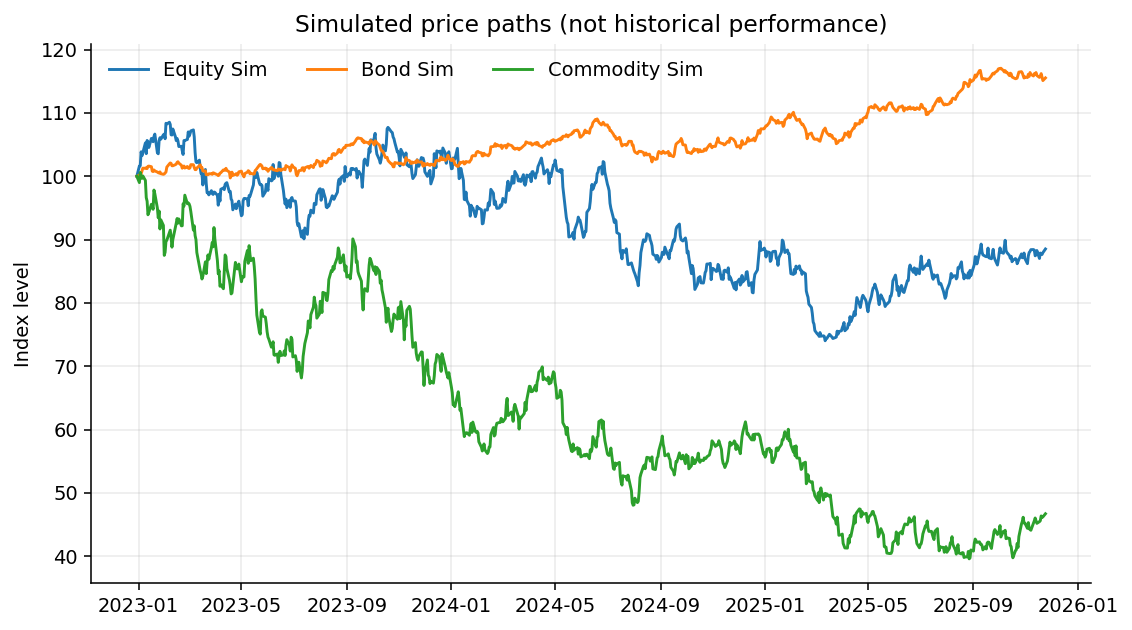
\includegraphics[width=0.94\textwidth]{simulated_paths.png}
  \caption{A reproducible set of simulated price paths. The paths are not historical observations or an investment forecast.}
\end{figure}

\begin{figure}[htbp]
  \centering
  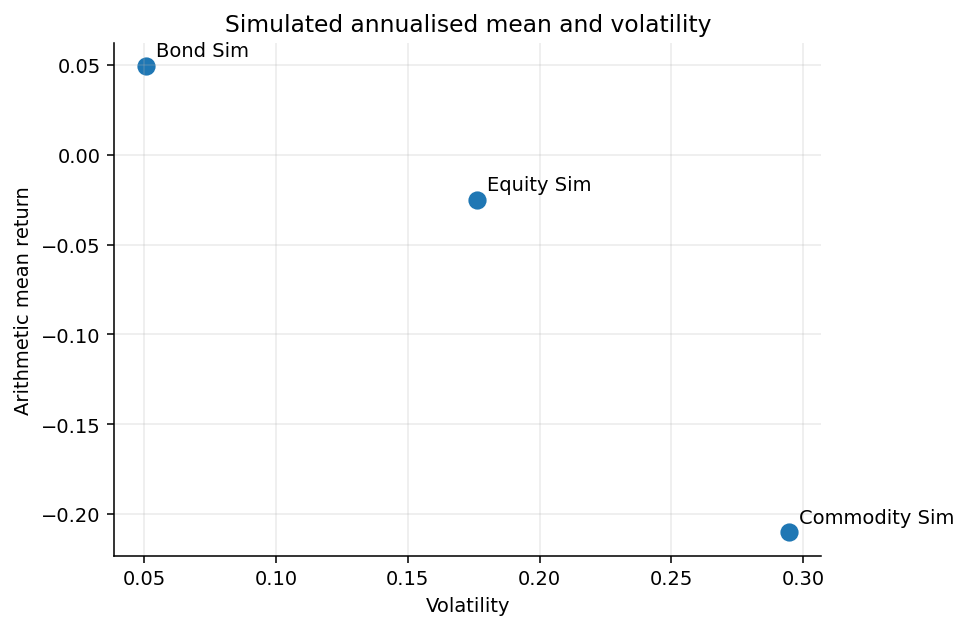
\includegraphics[width=0.78\textwidth]{simulated_risk_return.png}
  \caption{Arithmetic mean and volatility calculated from the same simulated returns. A sample point is not an expected-return claim.}
\end{figure}

\section{Using official data}
For a real research project, replace the simulated files only after recording a source, retrieval date, licensing terms, units, frequency, corporate-action treatment, and revision policy. The SEC publishes financial-statement data sets extracted from XBRL filings \cite{secdata}. TreasuryDirect documents Treasury marketable securities and their conventions \cite{treasury2026}. Central banks publish official rates and financial-stability reports. Provider permissions and rate limits apply.

\section{No performance guarantee}
Historical data can be revised, incomplete, or non-representative. A strategy's future return distribution is not known from its past sample. Even a correctly reproduced historical result can fail because the market, costs, participants, regulation, or strategy capacity changes.

\section{Reproduction command}
From the package root, create an environment with NumPy, pandas, matplotlib, and pytest or the Python standard-library test runner. Run:
\begin{verbatim}
python code/finance_models.py --generate-data \\
    --output-dir data --figure-dir figures
python -m unittest discover -s code -p 'test_*.py' -v
\end{verbatim}
The code uses a fixed seed for the supplied output. Changing the seed creates another simulated sample and should change the numerical results.

\chapter{Glossary}

\begin{description}
\item[Arbitrage] A strategy that has no initial net cost, no possible loss, and a positive gain in at least one state under stated assumptions.
\item[Asset] A controlled resource expected to provide future economic benefits.
\item[Basis] A difference between related spot and derivative prices; the sign convention must be stated.
\item[Beta] Covariance of an asset's return with a factor divided by factor variance.
\item[Bond] A debt claim promising contractual payments and principal under stated terms.
\item[Call option] The right, not obligation, to buy an underlying at a specified strike.
\item[Capital structure] The mix of debt, equity, and other financing claims.
\item[Clearing] Processes that calculate obligations, manage collateral, and support settlement.
\item[Convexity] Curvature of a price-yield or value-risk relationship.
\item[Correlation] Standardised linear dependence between two variables.
\item[Counterparty risk] Risk that the other party fails to perform.
\item[Coupon] Contractual interest payment on a bond.
\item[Credit spread] Yield or price compensation relative to a benchmark claim; not pure default probability.
\item[Derivative] A contract whose value depends on an underlying asset, rate, index, or event.
\item[Discount factor] Present value of one unit paid at a future date.
\item[Discount rate] Rate used to translate future cash flows into present value.
\item[Duration] A time-weighted or sensitivity-based measure of bond price exposure to yield.
\item[Efficient frontier] Feasible portfolios that are not dominated in expected return and risk under a chosen model.
\item[Equity] Residual ownership claim after liabilities.
\item[Expected shortfall] Average tail loss beyond a chosen loss quantile, under a defined distribution.
\item[Factor] A systematic return or state variable used to explain exposures.
\item[Forward] A private agreement to transact in the future at a fixed delivery price.
\item[Futures] A standardised, margined derivative usually marked to market daily.
\item[Gamma] Second derivative of derivative value with respect to underlying price.
\item[Hedging] Taking an offsetting position to reduce a defined exposure.
\item[Implied volatility] Volatility parameter that makes a model price equal an observed option price.
\item[Leverage] Exposure to assets or risks relative to equity or capital.
\item[Liquidity] Ability to transact or meet obligations with limited price impact or delay.
\item[Market capitalisation] Share price multiplied by shares outstanding.
\item[Market microstructure] Study of trading mechanisms, order flow, spreads, and price formation.
\item[Monte Carlo] Estimation by averaging outcomes from simulated random paths.
\item[Net asset value] Assets minus liabilities divided by units or shares of a pooled vehicle.
\item[No-arbitrage] Pricing principle that rules out exploitable riskless discrepancies under a model.
\item[Nominal return] Return measured in money prices before removing inflation.
\item[Option] A contingent right with nonlinear payoff.
\item[Portfolio] A collection of financial claims and their weights.
\item[Present value] Current equivalent value of future cash flows under a discounting convention.
\item[Put option] The right, not obligation, to sell an underlying at a specified strike.
\item[Risk premium] Expected compensation beyond a benchmark for bearing a risk or providing a service.
\item[Risk-neutral measure] A pricing probability measure under which appropriately discounted tradable prices are martingales.
\item[Sharpe ratio] Mean excess return divided by the standard deviation of excess return.
\item[Spot rate] Rate used to discount a single cash flow to a specific maturity.
\item[Stress test] Analysis of outcomes under a specified adverse scenario.
\item[Swap] Contract exchanging cash-flow streams, often based on rates, currencies, or commodities.
\item[Systemic risk] Risk that distress spreads through common exposures, interconnections, or feedback loops.
\item[Terminal value] Value assigned to cash flows beyond an explicit forecast horizon.
\item[Theta] Sensitivity of option value to the passage of time under a convention.
\item[Value at Risk] A loss quantile at a stated horizon and confidence level.
\item[Vega] Sensitivity of option value to the volatility input.
\item[Volatility] A measure of return dispersion, commonly standard deviation under a chosen horizon.
\end{description}

\chapter{Exercises and Solutions}

The questions appear at the end of the chapters. Solutions below show the method and a rounded result; a different result can be correct if the stated convention differs and is documented.

\section*{Chapters 1--4}
\begin{enumerate}
  \item[1.1] $(47-50+1.50)/50=-0.03$, so the return is -3 percent.
  \item[1.2] Accounting identity is a classification identity: assets equal the recorded claims on them. Market values can move without immediate accounting remeasurement.
  \item[1.3] $\E[R]=0.4(0.20)+0.6(-0.10)=0.02$. Variance is $0.4(0.18)^2+0.6(-0.12)^2=0.0144$, so volatility is 12 percent.
  \item[1.4] Funding, taxes, bid-ask spreads, short-sale constraints, margin, or counterparty default can prevent execution.
  \item[2.1] Primary market: the company sells newly issued shares and receives proceeds. Secondary market: investors trade existing shares and the company normally receives no proceeds.
  \item[2.2] It funds long-term activity with short-term claims, creating useful liquidity transformation but a mismatch if claims are withdrawn early.
  \item[2.3] Clearing can reduce bilateral settlement and replacement-cost exposure; it can concentrate default-fund, margin, operational, and liquidity risks at the central counterparty.
  \item[2.4] International standards require domestic legislation, supervision, and implementation choices.
  \item[3.1] Operating margin $=75/500=15\%$. ROE $=40/160=25\%$.
  \item[3.2] Receivables rising by 12 reduces CFO by 12; payables falling by 4 reduces CFO by 4. Total effect: CFO falls by 16.
  \item[3.3] $0.08(1.5)(2)=0.24$, or 24 percent.
  \item[3.4] Different accounting standards, lease treatment, asset age, intangibles, cyclicality, and market versus book values can change the ratio's meaning.
  \item[4.1] $10,000/1.06^4\approx7,920.94$.
  \item[4.2] Exact real return $=1.07/1.02-1\approx4.90\%$; approximation is 5 percent.
  \item[4.3] $NPV=-1000+600/1.1+600/1.1^2\approx41.32$.
  \item[4.4] The infinite growing cash-flow series converges only when $r>g$.
\end{enumerate}

\section*{Chapters 5--9}
\begin{enumerate}
  \item[5.1] $P=60/1.05+1,060/1.05^2\approx1,018.59$.
  \item[5.2] $\Delta P/P\approx-4.2(0.0025)=-1.05\%$.
  \item[5.3] Duration is linear; convexity captures the second-order curvature in the price-yield relationship.
  \item[5.4] $0.02(0.45)(5,000,000)=45,000$.
  \item[6.1] $3/(0.09-0.03)=50$.
  \item[6.2] $F=7(1.04)/(1.02)\approx7.1373$.
  \item[6.3] $(105-2)/10=10.30$ per unit.
  \item[6.4] Storage, financing, insurance, seasonality, and convenience yield can produce a positive carry even with flat expected spot.
  \item[7.1] Sunk cost: a feasibility study already paid for. Opportunity cost: rent forgone by using an owned building for the project.
  \item[7.2] No taxes and no distress costs are two assumptions. Bankruptcy costs make debt choice relevant.
  \item[7.3] $0.6(0.10)+0.4(0.05)(0.75)=0.075$, or 7.5 percent.
  \item[7.4] Staging creates the right to learn and expand only in favourable states, while avoiding some downside in unfavourable states.
  \item[8.1] $0.3(0.10)+0.7(-0.04)=0.002$, or 0.2 percent.
  \item[8.2] Uncorrelated variables can still have nonlinear dependence; independence implies zero correlation under finite moments, but the reverse is not true.
  \item[8.3] It is the model-implied change in expected excess return for a one-unit change in market excess return.
  \item[8.4] Some strategies will look significant by chance when many tests are run; the nominal 5 percent threshold no longer controls the family-wise error.
  \item[9.1] Variance $=0.5^2(0.20)^2+0.5^2(0.10)^2=0.0125$; volatility $\approx11.18\%$.
  \item[9.2] $\beta=0.018/0.0225=0.8$.
  \item[9.3] The factor model must be correctly specified and the error must be appropriately unrelated to the factor; otherwise the intercept can capture omitted risk or bias.
  \item[9.4] Expected returns and covariances are estimated with error; an unconstrained optimiser can exploit small estimation differences with extreme weights.
\end{enumerate}

\section*{Chapters 10--14}
\begin{enumerate}
  \item[10.1] Weak form concerns past market data; semi-strong form includes all public information.
  \item[10.2] Publication can lead to competition, arbitrage, changed trading costs, data-mining corrections, or a regime change.
  \item[10.3] A rule may be selected for fit, contain omitted variables, or depend on implementation assumptions; success alone does not identify a causal mechanism.
  \item[10.4] Sample period, universe, timing, benchmark, costs, turnover, capacity, and risk statistics are examples.
  \item[11.1] $Z$ is a standard-normal shock that generates the random terminal outcome.
  \item[11.2] $\mathbb Q$ is a pricing device that changes probabilities while preserving no-arbitrage pricing; it is not a claim about actual beliefs.
  \item[11.3] $0.008\sqrt{252}\approx0.1270$, or 12.70 percent.
  \item[11.4] The squared lagged shock increases the next conditional variance by $\alpha\varepsilon_{t-1}^2$.
  \item[12.1] $100e^{0.04(0.5)}\approx102.02$.
  \item[12.2] Initial margin is collateral against performance; losses can exceed it and variation margin can create further calls.
  \item[12.3] It scales the interest payments and therefore the exposure; principal is not necessarily exchanged.
  \item[12.4] Location mismatch and maturity mismatch are examples.
  \item[13.1] Call payoff is $\max(62-50,0)=12$; put payoff is zero.
  \item[13.2] Long stock plus a put replicates a call plus the present value of the strike, giving equality under no-arbitrage.
  \item[13.3] Hold half a share for each call and finance the remaining replicating position with the bond.
  \item[13.4] Real markets exhibit volatility smiles and skews; a single BSM parameter is an implied quote for each contract, not a universal constant.
  \item[14.1] Standard error falls as $1/\sqrt M$, so large accuracy gains require disproportionately more paths.
  \item[14.2] Position bounds, turnover limits, leverage caps, liquidity limits, and factor-neutrality constraints are examples.
  \item[14.3] Calibration error is mismatch between model and observed calibration targets; model error is the failure of the model structure to describe relevant reality.
  \item[14.4] Without timestamps, a researcher cannot verify that the signal used only information available at the decision time.
\end{enumerate}

\section*{Chapters 15--18}
\begin{enumerate}
  \item[15.1] VaR does not reveal the size or average of losses beyond the 99th percentile.
  \item[15.2] Market liquidity concerns trading without price impact; funding liquidity concerns meeting cash obligations.
  \item[15.3] A counterparty becomes weakest exactly when its obligation to you is largest, such as a derivative exposure rising as its credit spread widens.
  \item[15.4] A scenario preserves a coherent joint shock and can explore states not represented in a short historical sample.
  \item[16.1] Using an earnings number revised after the trading date is look-ahead bias.
  \item[16.2] A mid-price assumes immediate execution without paying the spread or moving the market; large orders cannot generally obtain it.
  \item[16.3] It is the largest percentage decline from a previous wealth peak to a later trough.
  \item[16.4] Kill switch, order-size limits, stale-data checks, reconciliation, audit logs, and incident response are examples.
  \item[17.1] Shock, margin call, forced sale, lower price/collateral, tighter funding, and further forced sale.
  \item[17.2] Insolvency means liabilities exceed asset value; illiquidity means obligations cannot be met when due, even if assets might cover them over time.
  \item[17.3] Questions include disparate error costs, explainability, appeal, privacy, data provenance, and whether users consented to the risk.
  \item[17.4] The label may use a narrow definition, omit transition risk, rely on poor data, or address impact rather than financial risk.
  \item[18.1] Build revenue and margin forecasts, calculate after-tax UFCF, discount each year, calculate terminal value, subtract net debt, and divide by shares.
  \item[18.2] Terminal value is highly sensitive when $WACC-g$ is small, so show a two-dimensional sensitivity and avoid false precision.
  \item[18.3] Review debt service, covenant headroom, refinancing, downside cash flows, and the value of flexibility.
  \item[18.4] Compare marginal contribution to portfolio return, covariance, factor exposure, liquidity, and concentration rather than standalone return alone.
\end{enumerate}



\backmatter

\chapter*{Bibliography}
\addcontentsline{toc}{chapter}{Bibliography}
\begin{thebibliography}{99}

\bibitem{arrow1964}
Arrow, K. J. (1964). \textit{The Role of Securities in the Optimal Allocation of Risk-Bearing}. Review of Economic Studies, 31(2), 91--96. doi:10.2307/2296188.

\bibitem{basel2019}
Basel Committee on Banking Supervision. (2019, current framework consulted 2026). \textit{Minimum capital requirements for market risk}. Bank for International Settlements. \url{https://www.bis.org/bcbs/publ/d457.htm}

\bibitem{basel3}
Basel Committee on Banking Supervision. (2017, framework current 2026). \textit{Basel III: Finalising post-crisis reforms}. Bank for International Settlements. \url{https://www.bis.org/bcbs/publ/d424.htm}

\bibitem{blackscholes1973}
Black, F., and Scholes, M. (1973). The pricing of options and corporate liabilities. \textit{Journal of Political Economy}, 81(3), 637--654. doi:10.1086/260062.

\bibitem{bollerslev1986}
Bollerslev, T. (1986). Generalized autoregressive conditional heteroskedasticity. \textit{Journal of Econometrics}, 31(3), 307--327. doi:10.1016/0304-4076(86)90063-1.

\bibitem{cftc2026}
U.S. Commodity Futures Trading Commission. (2026). \textit{Futures market basics}. \url{https://www.cftc.gov/LearnAndProtect/AdvisoriesAndArticles/FuturesMarketBasics/index.htm}

\bibitem{cochrane2005}
Cochrane, J. H. (2005). \textit{Asset Pricing}. Revised edition. Princeton University Press.

\bibitem{cont2001}
Cont, R. (2001). Empirical properties of asset returns: Stylized facts and statistical issues. \textit{Quantitative Finance}, 1(2), 223--236. doi:10.1080/713665670.

\bibitem{ecb2026}
European Central Bank. (2026, May 19). \textit{Financial Stability Review}. \url{https://www.ecb.europa.eu/press/financial-stability-publications/fsr/html/ecb.fsr202605~50566915a7.en.html}

\bibitem{engle1982}
Engle, R. F. (1982). Autoregressive conditional heteroscedasticity with estimates of the variance of United Kingdom inflation. \textit{Econometrica}, 50(4), 987--1007. doi:10.2307/1912773.

\bibitem{fama1970}
Fama, E. F. (1970). Efficient capital markets: A review of theory and empirical work. \textit{Journal of Finance}, 25(2), 383--417. doi:10.2307/2325486.

\bibitem{famafrench1993}
Fama, E. F., and French, K. R. (1993). Common risk factors in the returns on stocks and bonds. \textit{Journal of Financial Economics}, 33(1), 3--56. doi:10.1016/0304-405X(93)90023-5.

\bibitem{famafrench2015}
Fama, E. F., and French, K. R. (2015). A five-factor asset pricing model. \textit{Journal of Financial Economics}, 116(1), 1--22. doi:10.1016/j.jfineco.2014.10.010.

\bibitem{federalreserve2025}
Board of Governors of the Federal Reserve System. (2025). \textit{Financial Stability Report}. \url{https://www.federalreserve.gov/publications/financial-stability-report.htm}

\bibitem{hull2022}
Hull, J. C. (2022). \textit{Options, Futures, and Other Derivatives} (11th ed.). Pearson.

\bibitem{ianes2011}
International Organization of Securities Commissions. (2011). \textit{Principles for Financial Market Infrastructures}. Committee on Payment and Settlement Systems and Technical Committee of IOSCO. \url{https://www.bis.org/cpmi/publ/d101a.pdf}

\bibitem{jensen1968}
Jensen, M. C. (1968). The performance of mutual funds in the period 1945--1964. \textit{Journal of Finance}, 23(2), 389--416. doi:10.2307/2325404.

\bibitem{kahneman1979}
Kahneman, D., and Tversky, A. (1979). Prospect theory: An analysis of decision under risk. \textit{Econometrica}, 47(2), 263--291. doi:10.2307/1914185.

\bibitem{kelly1956}
Kelly, J. L. (1956). A new interpretation of information rate. \textit{Bell System Technical Journal}, 35(4), 917--926. doi:10.1002/j.1538-7305.1956.tb03809.x.

\bibitem{lakonishok1994}
Lakonishok, J., Shleifer, A., and Vishny, R. W. (1994). Contrarian investment, extrapolation, and risk. \textit{Journal of Finance}, 49(5), 1541--1578. doi:10.2307/2329452.

\bibitem{merton1973}
Merton, R. C. (1973). Theory of rational option pricing. \textit{Bell Journal of Economics and Management Science}, 4(1), 141--183. doi:10.2307/3003143.

\bibitem{modigliani1958}
Modigliani, F., and Miller, M. H. (1958). The cost of capital, corporation finance and the theory of investment. \textit{American Economic Review}, 48(3), 261--297.

\bibitem{modigliani1963}
Modigliani, F., and Miller, M. H. (1963). Corporate income taxes and the cost of capital: A correction. \textit{American Economic Review}, 53(3), 433--443.

\bibitem{markowitz1952}
Markowitz, H. (1952). Portfolio selection. \textit{Journal of Finance}, 7(1), 77--91. doi:10.2307/2975974.

\bibitem{mcfadden1974}
McFadden, D. (1974). Conditional logit analysis of qualitative choice behavior. In P. Zarembka (ed.), \textit{Frontiers in Econometrics}. Academic Press.

\bibitem{mishkin2019}
Mishkin, F. S. (2019). \textit{The Economics of Money, Banking, and Financial Markets} (12th ed.). Pearson.

\bibitem{secfinancialstatements}
U.S. Securities and Exchange Commission. (2007). \textit{Beginner's guide to financial statements}. \url{https://www.sec.gov/about/reports-publications/investorpubsbegfinstmtguide}

\bibitem{sec10k}
U.S. Securities and Exchange Commission. (2021). \textit{How to read a 10-K/10-Q}. \url{https://www.sec.gov/resources-for-investors/investor-alerts-bulletins/how-read-10-k10-q}

\bibitem{secdata}
U.S. Securities and Exchange Commission. (2026). \textit{Financial statement data sets}. \url{https://www.sec.gov/data-research/sec-markets-data/financial-statement-data-sets}

\bibitem{sharpe1964}
Sharpe, W. F. (1964). Capital asset prices: A theory of market equilibrium under conditions of risk. \textit{Journal of Finance}, 19(3), 425--442. doi:10.2307/2977928.

\bibitem{shiller1981}
Shiller, R. J. (1981). Do stock prices move too much to be justified by subsequent changes in dividends? \textit{American Economic Review}, 71(3), 421--436.

\bibitem{sortino1994}
Sortino, F. A., and Price, L. N. (1994). Performance measurement in a downside risk framework. \textit{Journal of Investing}, 3(3), 59--64.

\bibitem{treasury2026}
U.S. Department of the Treasury. (2026). \textit{Marketable securities and glossary}. TreasuryDirect. \url{https://www.treasurydirect.gov/marketable-securities/}

\bibitem{tsay2010}
Tsay, R. S. (2010). \textit{Analysis of Financial Time Series} (3rd ed.). Wiley.

\bibitem{white2000}
White, H. (2000). A reality check for data snooping. \textit{Econometrica}, 68(5), 1097--1126. doi:10.2307/2999436.

\end{thebibliography}

\printindex

\end{document}
